\documentclass[a4paper, 12pt]{report}
\usepackage[utf8]{inputenc}
\usepackage{amsmath}
\usepackage{xcolor}
\usepackage{hyperref}
\usepackage{graphicx}
\usepackage{booktabs}
\usepackage{shadowtext}

\hypersetup{
	colorlinks=true,       % Enable colored links
	linkcolor=blue,        % Color for internal links (e.g., sections, figures)
	filecolor=magenta,     % Color for file links
	urlcolor=cyan,         % Color for URLs
	citecolor=blue,       % Color for citations
}

\usepackage{geometry}
\usepackage{cite}

\usepackage{fancyhdr} % For running headers

\pagestyle{fancy}
\fancyhf{} % Clear default settings
\fancyhead[LO]{\leftmark} % Left-side header (odd pages)
\fancyhead[RE]{\rightmark} % Right-side header (even pages)
\fancyfoot[C]{\thepage} % Page number at the center footer

\geometry{margin=1in}

\begin{document}
	
	\begin{titlepage}
	\centering
	\vfill % Push content down
	
	{\Large \textsc{A Project Report}\par}
	\vspace{0.5cm}
	{\normalsize on\par}
	\vspace{0.5cm}
	{\huge \textsc{Time Series Machine Learning}\par} % Updated project title
	\vspace{1cm}
	{\normalsize Submitted to\par}
	\vspace{0.5cm}
	{\Large \textsc{KIIT Deemed to be University}\par}
	\vspace{1cm}
	{\normalsize In Partial Fulfilment of the Requirement for the Award of\par}
	\vspace{0.5cm}
	{\Large \textsc{Bachelor's Degree in \\ Computer Science \& Engineering}\par}
	\vspace{1cm}
	{\normalsize BY\par}
	\vspace{0.5cm}
	\begin{tabular}{ll}
		\textsc{Adarsh Narayan} & \textsc{22052352} \\
		\textsc{Akash Kumar}    & \textsc{22051659} \\
		\textsc{Aman Pathak}    & \textsc{22051662} \\
		\textsc{Amit Kumar}     & \textsc{22053747} \\
	\end{tabular}
	\par
	\vspace{0.5cm}
	{\normalsize UNDER THE GUIDANCE OF\par}
	\vspace{0.5cm}
	{\normalsize Prof.~Jyotiprakash \textsc{Mishra}\par}
	
	\vfill % Push content upwards to center everything
	
	
\includegraphics[width=0.15\textwidth]{./assets/bw_kiit.png}\par % Logo at the bottom
\end{titlepage}

	
	\newpage
	\begin{center}
		\Large \textbf{SCHOOL OF COMPUTER ENGINEERING} \\[0.5cm]
		\Large \textbf{KALINGA INSTITUTE OF INDUSTRIAL TECHNOLOGY} \\[0.5cm]
		\large BHUBANESWAR, ODISHA - 751024 \\[1cm]
		\large April 2025
	\end{center}
	
	\newpage
\begin{center}
	\Large \textbf{Acknowledgements}
\end{center}
\vspace{1cm}

\noindent
We would like to express our sincere gratitude to our guide, Dr.~Jyotiprakash \textsc{Mishra}, for his invaluable guidance, support, and encouragement throughout this project. We also extend our thanks to the faculty members of the School of Computer Engineering, KIIT Deemed to be University, for their insightful lectures and constant motivation. Lastly, we are grateful to our families and friends for their continuous support and encouragement.

\vspace{2cm}

\vspace{1cm}

\noindent
\rule{6cm}{0.4pt} \\ 
Adarsh Narayan \\[1cm]

\noindent
\rule{6cm}{0.4pt} \\ 
Akash Kumar \\[1cm]

\noindent
\rule{6cm}{0.4pt} \\ 
Aman Pathak \\[1cm]

\noindent
\rule{6cm}{0.4pt} \\ 
Amit Kumar

	

	\newpage
\begin{center}
	\Large \textbf{Abstract}
\end{center}
\vspace{1cm}

\noindent
Time series forecasting plays a crucial role in various domains, enabling accurate predictions based on historical patterns. This project explores different time series machine learning techniques applied to four diverse datasets, each addressing a unique problem statement. The first dataset, Household Power Consumption, involves forecasting hourly and daily energy usage patterns to enhance energy efficiency. The second dataset, Predictive Maintenance, focuses on detecting potential machine failures using sensor data, contributing to proactive maintenance strategies. The third dataset, Walmart and Rossmann Store Sales, aims to predict retail sales while accounting for seasonal trends, promotional effects, and holidays. Lastly, the Historical Stock Market Data dataset is used to predict closing prices and identify potential trading signals, assisting in financial decision-making.  

\vspace{0.5cm}

\noindent
The project follows a structured approach, beginning with data wrangling techniques such as timestamp conversion, handling missing data, and resampling to maintain consistency. Feature engineering is employed to enhance predictive performance, incorporating moving averages, rolling windows, and external data sources like holidays, weather conditions, and macroeconomic indicators. A comprehensive model comparison is conducted, evaluating traditional statistical models (ARIMA/SARIMA), machine learning methods (Random Forest, XGBoost), and deep learning architectures (LSTM, GRU). Model performance is assessed using error metrics such as Mean Squared Error (MSE), Root Mean Squared Error (RMSE), Mean Absolute Error (MAE), and Mean Absolute Percentage Error (MAPE). Additionally, explainability techniques such as SHAP values and feature importance plots are applied to ensemble models, providing insights into the key drivers of predictions. Visualizations, including forecasted vs. actual values, seasonal trends, and anomaly detection, further illustrate the effectiveness of the chosen models. The results highlight the strengths and limitations of various approaches, demonstrating the applicability of machine learning and deep learning models in real-world time series forecasting problems.

\vfill

	
	
	\tableofcontents
	
	\chapter{Time Series Machine Learning for Household Power Consumption}

	\section{Introduction to Machine Learning}
	Machine Learning (ML) is a subset of artificial intelligence that enables systems to learn from data and improve over time without explicit programming. In this chapter, we explore ML techniques applied to time series forecasting, specifically for predicting household power consumption. This section delves into the definitions, sub-categories, related fields, and practical applications of ML, setting the stage for its application to our problem.
	
	\subsection{Definitions of Machine Learning}
	Machine learning has been defined by multiple scholars in related ways, emphasizing its reliance on data and experience. Tom Mitchell, in his seminal work \textit{Machine Learning} \cite{mitchell1997machine}, provides a formal definition:
	\begin{quote}
		A computer program is said to learn from experience $E$ with respect to some class of tasks $T$ and performance measure $P$, if its performance at tasks in $T$, as measured by $P$, improves with experience $E$.
	\end{quote}
	This definition encapsulates algorithms like gradient descent and Q-learning, where performance improves through iterative exposure to data.
	
	Kevin Murphy, in \textit{Machine Learning: A Probabilistic Perspective} \cite{murphy2012machine}, describes ML as:
	\begin{quote}
		A set of methods that can automatically detect patterns in data, and then use the uncovered patterns to predict future data, or to perform other kinds of decision making under uncertainty (such as planning how to collect more data!).
	\end{quote}
	This highlights ML's predictive and decision-making capabilities.
	
	Shalev-Shwartz and Ben-David offer a simpler perspective \cite{shalev2014understanding}:
	\begin{quote}
		The term machine learning refers to the automated detection of meaningful patterns in data.
	\end{quote}
	Across these definitions, the core concept is data-driven pattern recognition to solve tasks. However, the term ``automatically'' can mislead; ML algorithms typically require human-defined performance measures and parameters, indicating they are not fully autonomous.
	
	As a field, ML can be defined as the study and application of such algorithms, aligning with Mitchell's framework.
	
	\subsection{Sub-Categories of Machine Learning}
	Machine learning is often divided into three primary sub-categories, as noted by Murphy and others \cite{murphy2012machine}:
	\begin{itemize}
		\item \textbf{Supervised Learning (Predictive):} The goal is to learn a mapping from inputs $x$ to outputs $y$, given labeled input-output pairs. For our household power consumption problem, this involves predicting energy usage from historical data.
		\item \textbf{Unsupervised Learning (Descriptive):} This seeks to find interesting patterns in data without predefined labels, such as clustering consumption trends.
		\item \textbf{Reinforcement Learning:} Useful for learning optimal actions based on occasional reward or punishment signals, less relevant here but notable in broader ML contexts.
	\end{itemize}
	
	Additional sub-categories or taxonomies include:
	\begin{itemize}
		\item \textbf{Deep Learning:} Utilizes neural networks and algorithms like gradient descent to approximate complex functions, critical for later sections on RNNs and LSTMs.
		\item \textbf{Probabilistic Machine Learning:} Offers uncertainty estimation, enhancing forecast reliability.
		\item \textbf{Weakly Supervised Learning:} Addresses imperfect labels, a potential challenge in noisy datasets.
		\item \textbf{Online Learning:} Processes one data point at a time, contrasting with batch learning from datasets.
	\end{itemize}
	These can intersect, e.g., deep learning can be online or offline, offering flexibility in application.
	
	\subsection{Related Fields}
	A closely related field is \textit{computational (or statistical) learning theory}, which examines the theoretical underpinnings of learning from computational and statistical perspectives. It addresses questions like, ``How many samples are needed to approximate a function with a given error?''
	
	ML also overlaps with statistics, adopting concepts like regression and hypothesis testing. While some quip that ML is ``glorified statistics,'' the fields differ in focus: statistics emphasizes inference and modeling, while ML prioritizes prediction and automation. For a deeper comparison, see \cite{bzdok2018statistics}.
	
	\subsection{Applications of Machine Learning}
	ML excels at automating tasks involving data and pattern recognition, historically human-dominated, such as language translation or image classification. In our context, it enables forecasting hourly or daily household power consumption from the UCI dataset (\url{https://archive.ics.uci.edu/ml/datasets/individual+household+electric+power+consumption}).
	
	However, ML has limitations. It cannot inherently infer causal relationships from data—causal inference, as explored by Judea Pearl \cite{pearl2009causal}, requires additional frameworks. Thus, while ML can predict energy usage, understanding \textit{why} usage changes may need human insight or causal methods.
	
	\subsection{Relevance to Time Series Forecasting}
	For our goal of forecasting household power consumption, ML offers tools to detect temporal patterns and predict future usage. Supervised learning, deep learning (e.g., LSTMs), and feature importance analysis (e.g., SHAP) will be pivotal, bridging general ML concepts to time series specifics in subsequent sections.
		
	\section{Differences Between Time Series and Machine Learning}
	While traditional machine learning (ML) often assumes independent and identically distributed (i.i.d.) data, time series data is inherently sequential and autocorrelated. This distinction necessitates specialized techniques for modeling temporal dependencies. In traditional ML, algorithms such as support vector machines, decision trees, or neural networks are designed to handle data where the order of observations does not matter, and each data point is assumed to be drawn independently from the same distribution. However, time series data—such as stock prices, weather measurements, or sensor readings—exhibits temporal structure, where the value at a given time step is often dependent on previous observations. This autocorrelation violates the i.i.d. assumption, rendering standard ML approaches less effective unless adapted appropriately.
	
	To address these challenges, time series analysis employs techniques that explicitly model temporal relationships. For instance, classical methods like ARIMA (AutoRegressive Integrated Moving Average) capture trends, seasonality, and lagged dependencies in the data. In contrast, machine learning approaches can be extended to time series by incorporating sequential modeling techniques, such as recurrent neural networks (RNNs) or transformers, which are designed to process ordered data. Libraries like \texttt{sktime} provide a unified framework for adapting ML algorithms—e.g., regression models or gradient boosting—to time series tasks, such as forecasting, by treating temporal data as a supervised learning problem where past values predict future ones. 
	
	A key difference lies in the evaluation and preprocessing requirements. Time series modeling often requires stationarity checks, differencing, or decomposition to handle trends and seasonality, whereas traditional ML focuses on feature engineering and cross-validation without regard to temporal ordering. Moreover, splitting data for training and testing in time series must preserve chronological order to avoid data leakage, unlike the random shuffling common in i.i.d. settings. Thus, while ML offers flexibility and scalability, time series analysis provides domain-specific tools to capture the unique dynamics of sequential data, often requiring a hybrid approach for optimal performance.

	\section{Autoregression}
	Autoregression (AR) models are a class of statistical tools used to predict future values of a time series based on a linear combination of its past observations. These models assume that the current value of the series can be expressed as a weighted sum of previous values, plus a random error term. This approach is particularly effective for capturing temporal dependencies in data, making it well-suited for applications like forecasting power consumption, where historical patterns often influence future behavior. In the context of power consumption, an AR model might leverage daily or hourly usage data to identify trends, seasonality, or recurring cycles, such as increased demand during peak hours. By estimating the coefficients of the linear combination through methods like least squares, the model provides a simple yet powerful framework for short-term predictions, adaptable to stationary time series or stabilized data.
	
	\section{Sliding Window}
	In the context of time series analysis, the sliding window approach is a widely used technique to prepare data for training predictive models. This method involves creating fixed-size input-output pairs from a time series dataset to enable a model to learn temporal patterns and make predictions. The ``window'' refers to a contiguous subset of the time series data, which is moved (or ``slid'') across the entire sequence step-by-step. At each step, the data within the window forms an input-output pair: the input consists of a fixed number of consecutive observations (often called the ``look-back period''), and the output is typically the next value or values in the sequence (the ``prediction horizon'').
	
	For example, consider a time series of daily temperature readings denoted as 
	
	\[ \{T_1, T_2, T_3, T_4, T_5, T_6, \dots\} \].
	
	If we define a window size of 3 for the input and 1 for the output, the sliding window process generates pairs such as:
	\begin{itemize}
		\item Input: \( [T_1, T_2, T_3] \), Output: \( T_4 \)
		\item Input: \( [T_2, T_3, T_4] \), Output: \( T_5 \)
		\item Input: \( [T_3, T_4, T_5] \), Output: \( T_6 \)
	\end{itemize}
	The window slides forward by a fixed step size (commonly one time step, though larger steps can be used to reduce overlap), systematically covering the entire time series. This transforms the sequential data into a supervised learning problem, where the model learns to map the input window (past observations) to the output (future value(s)), expressed as:
	\[
	f([T_t, T_{t+1}, T_{t+2}]) \rightarrow T_{t+3}
	\]
	where \( t \) represents the starting time index of the window.
	
	This approach is particularly useful for training machine learning models, such as neural networks, autoregressive models, or traditional statistical methods, on time series data. The size of the window is a critical hyperparameter: a smaller window may capture short-term patterns, while a larger window can incorporate longer-term dependencies. Additionally, the method can be adapted to multi-step forecasting by setting the output to include multiple future values, e.g., \( [T_{t+3}, T_{t+4}] \) instead of just \( T_{t+3} \).
	
	By sliding the window across the time series, this technique maximizes the use of available data, creating numerous training examples even from a single sequence. This makes it an efficient and flexible strategy for modeling temporal dynamics in applications such as finance, weather forecasting, or signal processing.

	\subsection{Predicting Target or Differences}
	In this section, we investigate two distinct approaches to modeling power consumption: predicting the raw power consumption values directly versus predicting the differences between consecutive power consumption values. Each method presents unique advantages and challenges, and our analysis focuses on evaluating the trade-offs in terms of accuracy, stability, and practical applicability.
	
	Predicting raw power consumption values involves training a model to estimate the absolute power usage at each time step based on relevant input features, such as historical data, environmental conditions, or system load. This approach has the benefit of directly providing interpretable outputs that align with real-world measurements, making it intuitive for downstream applications like energy monitoring or resource planning. However, it can be sensitive to trends, seasonality, or abrupt shifts in the data, which may lead to cumulative errors or reduced robustness, especially in the presence of noise or outliers.
	
	In contrast, predicting the differences—often referred to as a differential or delta-based approach—focuses on modeling the change in power consumption between consecutive time steps rather than the absolute values. This method can mitigate issues related to long-term trends or baseline shifts, as it inherently emphasizes short-term variations. By capturing these incremental changes, the model may achieve greater stability in scenarios where the data exhibits high variability or non-stationarity. However, a key trade-off is that errors in predicting differences can accumulate when reconstructing the raw values, potentially leading to drift over time. Additionally, this approach may require an additional step to integrate the predicted differences with an initial value to recover the absolute power consumption, introducing complexity in implementation.
	
	To assess these approaches, we compare their performance across metrics such as mean absolute error (MAE) for accuracy and variance of predictions for stability. We also consider the computational overhead and the ease of integrating each method into real-time systems. Our analysis aims to determine under what conditions—such as data characteristics, prediction horizon, or application requirements—one approach outperforms the other, providing insights into their suitability for different use cases in power consumption forecasting.
	
	\subsection{Intuition Behind First Differences}
	
	The first difference of a time series, defined as \(\Delta x_t = x_t - x_{t-1}\), is akin to a discrete derivative, capturing the rate of change between consecutive observations. This transformation is a fundamental technique in time series analysis, particularly for stabilizing non-stationary series to make them more amenable to modeling. By focusing on changes rather than absolute values, differencing can remove trends and other non-stationary components, enabling the application of statistical tools designed for stationary processes.
	
	Differencing is especially appropriate when a time series \(\{x_t\}\) contains one or more unit roots, meaning it is integrated of order \(d = 1, 2, \ldots\), denoted as \(I(d)\). A series with unit roots exhibits non-stationarity, such as a random walk or higher-order cumulative sums, and its statistical properties (e.g., mean and variance) evolve over time. The goal of differencing is to reduce the order of integration until the resulting series is \(I(0)\), which is approximately stationary and thus benefits from a wealth of statistical results derived for such processes.
	
	For an \(I(1)\) series, which has a single unit root, \(\{x_t\}\) can be expressed as a cumulative sum of an \(I(0)\) time series: \(x_t = \sum_{\tau=1}^t u_\tau\), where \(\{u_\tau\}\) is \(I(0)\), meaning it has a constant mean and variance. A classic example is a logarithmic stock price, \(\{p_t\} = \{\ln(P_t)\}\), where the logarithmic returns, \(\{\ln(P_t / P_{t-1})\} = \{p_t - p_{t-1}\}\), are approximately \(I(0)\). Taking the first difference of an \(I(1)\) series, \(\Delta x_t = x_t - x_{t-1}\), yields an \(I(0)\) series, which is convenient for modeling because stationary processes have well-established properties, such as ergodicity and predictable autocorrelation structures. While an \(I(0)\) series is not identical to a strictly stationary one---due to potential heteroskedasticity or other subtle deviations---the approximation is often sufficient for practical purposes.
	
	For an \(I(2)\) series, which has two unit roots, the first-differenced series \(\{\Delta x_t\}\) remains \(I(1)\), and a second difference, \(\Delta^2 x_t = \Delta x_t - \Delta x_{t-1}\), is required to reach \(I(0)\). Here, the original series can be viewed as a ``twice-cumulative sum'' of an \(I(0)\) process: \(x_t = \sum_{\tau=1}^t \left( \sum_{s=1}^\tau v_s \right)\), where \(\{v_s\}\) is \(I(0)\). Some economists suggest that the consumer price index (CPI) approximates an \(I(2)\) process, implying that price increments (i.e., inflation rates) are \(I(1)\). This reflects the persistence often observed in inflation data, though the adequacy of this approximation remains a subject of debate among researchers due to varying empirical evidence.
	
	Higher-order integration, such as \(I(3)\), is theoretically possible but rare in real-world data. I am not aware of any widely recognized \(I(3)\) processes in practice, as most economic or physical time series are adequately described by \(I(1)\) or \(I(2)\) models.
	
	Care must be taken when applying differencing, as overdifferencing an \(I(d)\) series---i.e., differencing it more than \(d\) times---can introduce problems. Overdifferencing increases the error variance of the model compared to one with the appropriate order of differencing (\(d\)) and induces a moving-average component with a negative unit root in the resulting series. This can complicate forecasting and degrade model performance. For example, differencing an \(I(0)\) series once produces an \(I(-1)\) series, which is overstationary and exhibits undesirable properties like increased noise. Thus, differencing should be applied judiciously, typically guided by tests for unit roots (e.g., the Augmented Dickey-Fuller test) to determine the correct order \(d\).
	
	\section{Data Preparation and Analysis}
	
	\subsection{Cleaning the Dataset}
	The dataset, comprising power consumption metrics such as global active power, reactive power, voltage, and sub-metering readings, requires preprocessing to ensure data quality for subsequent modeling. Initially, the raw data is loaded from a text file with separate date and time fields, which are combined into a unified datetime format to facilitate time-based analysis. Missing values, often represented by special characters or undefined entries, are identified and addressed through linear interpolation, ensuring continuity in the time series. This step mitigates the impact of gaps that could skew statistical analyses or predictive models. Additionally, data types are explicitly defined to maintain consistency, converting relevant columns to numerical formats suitable for computation. A subset of the data, representing the first 2.5\% of the records, is extracted alongside the full dataset for comparative analysis, enabling efficient testing on a smaller scale while preserving the integrity of the complete dataset.
	
	\subsection{Exploratory Data Analysis}
	Exploratory data analysis (EDA) is conducted to uncover underlying patterns, trends, and anomalies within the power consumption data. Basic statistical summaries, including measures of central tendency and dispersion, are calculated to provide an overview of the dataset's characteristics. The presence of missing values is quantified to assess data completeness post-cleaning. Visualizations play a critical role in this phase, offering insights into temporal dynamics. A time series plot of global active power reveals fluctuations over time, highlighting potential daily or seasonal patterns (see Figure~\ref{fig:global_active_power}). Voltage trends are similarly examined, displaying stability or variability across the observation period (see Figure~\ref{fig:voltage_trends}). Consumption patterns across three sub-metering categories are visualized to compare their individual contributions to total energy usage, with overlapping trends indicating distinct usage behaviors (see Figure~\ref{fig:sub_metering}). To further explore variability, rolling statistics—such as a 50-point mean and standard deviation—are computed and plotted alongside the original global active power data, smoothing short-term fluctuations and exposing longer-term trends (see Figure~\ref{fig:rolling_stats}). Finally, a seasonal decomposition is performed on the global active power series, separating it into trend, seasonal, and residual components, with a daily periodicity assumption (e.g., 1440 minutes), to quantify recurring patterns and noise (see Figure~\ref{fig:decomposition_full}).
	
	\begin{figure}[htbp]
		\centering
		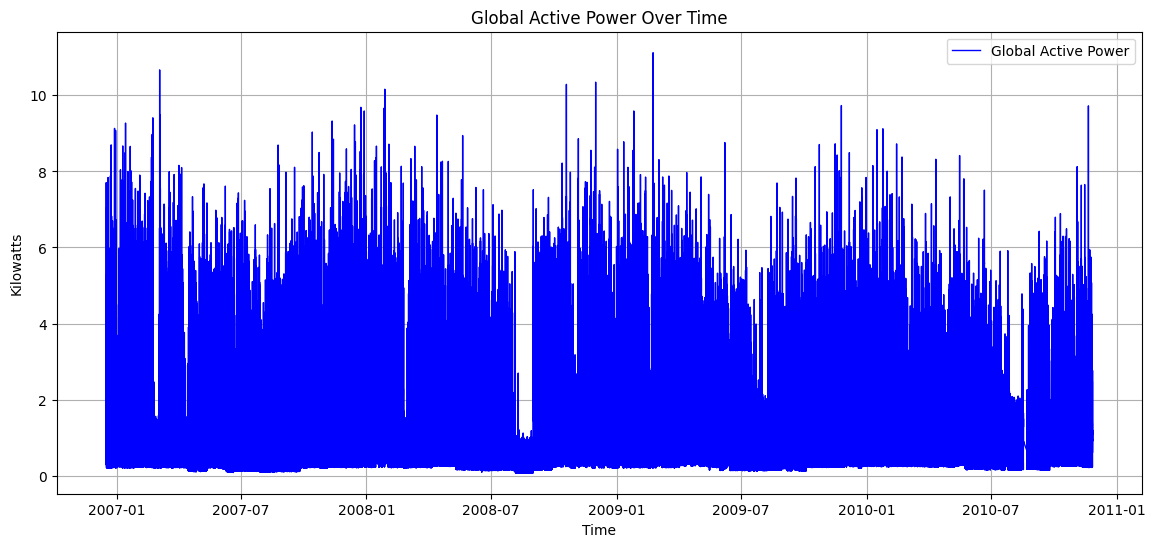
\includegraphics[width=0.7\textwidth]{./figures_aman/global_active_power_over_time.png}
		\caption{Global Active Power Over Time}
		\label{fig:global_active_power}
	\end{figure}
	
	\begin{figure}[htbp]
		\centering
		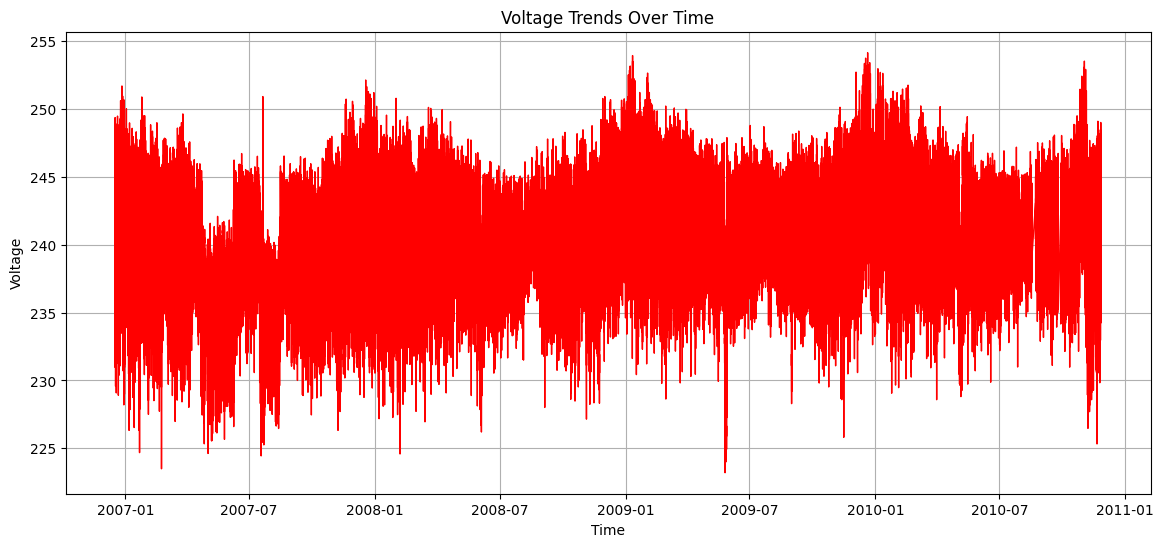
\includegraphics[width=0.9\textwidth]{./figures_aman/voltage_trends_over_time.png}
		\caption{Voltage Trends Over Time}
		\label{fig:voltage_trends}
	\end{figure}
	
	\begin{figure}[htbp]
		\centering
		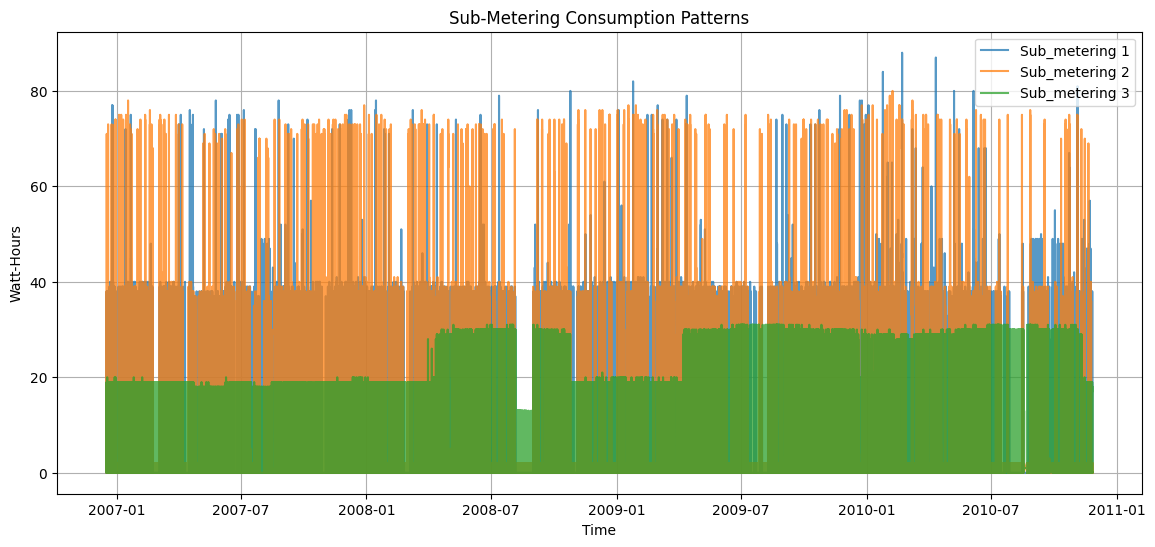
\includegraphics[width=0.7\textwidth]{./figures_aman/sub_metering_patterns.png}
		\caption{Sub-Metering Consumption Patterns}
		\label{fig:sub_metering}
	\end{figure}
	
	\begin{figure}[htbp]
		\centering
		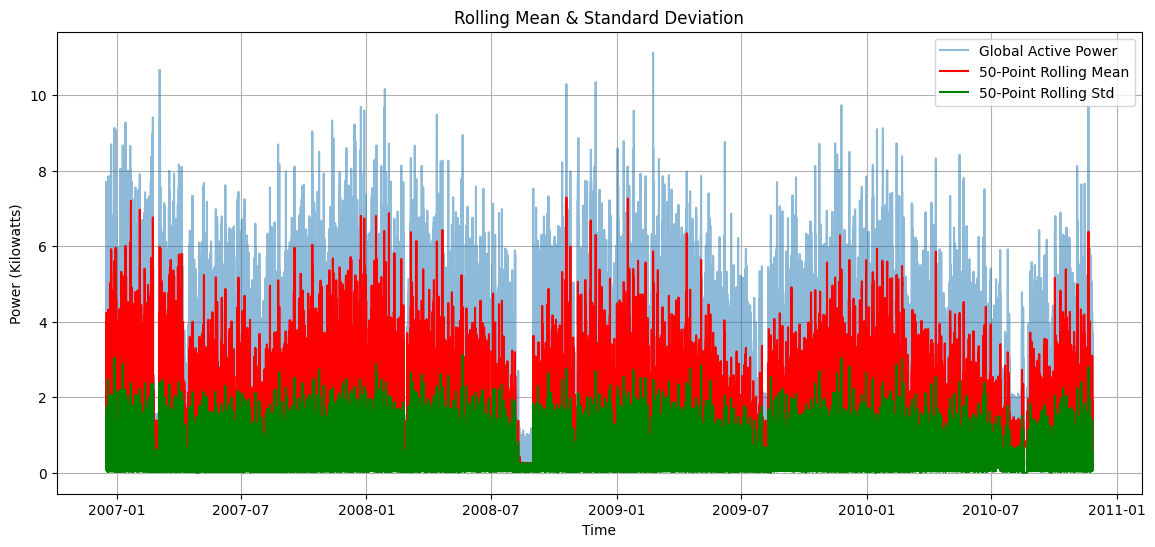
\includegraphics[width=0.7\textwidth]{./figures_aman/rolling_mean_std.png}
		\caption{Rolling Mean and Standard Deviation of Global Active Power}
		\label{fig:rolling_stats}
	\end{figure}
	
	\begin{figure}[htbp]
		\centering
		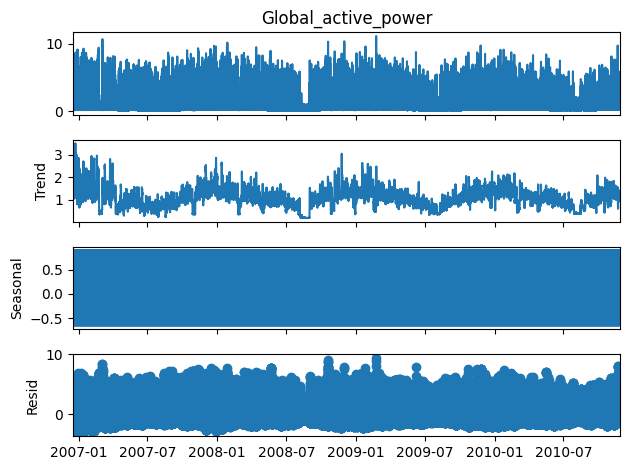
\includegraphics[width=0.7\textwidth]{./figures_aman/seasonal_decomposition_full.png}
		\caption{Seasonal Decomposition of Global Active Power (Full Dataset)}
		\label{fig:decomposition_full}
	\end{figure}
	
	\subsection{Resampling by Time Unit}
	To enable forecasting at different temporal resolutions, the dataset is resampled from its original granularity to hourly, daily, weekly, and monthly intervals. For hourly aggregation, sub-hourly measurements are summed, creating a coarser time series that captures total energy consumption within each hour. This process is applied to both the full dataset and its subset, preserving consistency across analyses. The resampled hourly data is saved for further use, facilitating predictions of energy usage at practical time scales. Beyond hourly resampling, daily, weekly, and monthly averages are computed to explore longer-term trends. For instance, a plot of daily global active power illustrates smoothed consumption patterns, reducing noise and emphasizing day-to-day variations (see Figure~\ref{fig:daily_power}). These resampled datasets provide flexibility in modeling, catering to diverse forecasting needs, from short-term operational planning to long-term energy management.
	
	\begin{figure}[htbp]
		\centering
		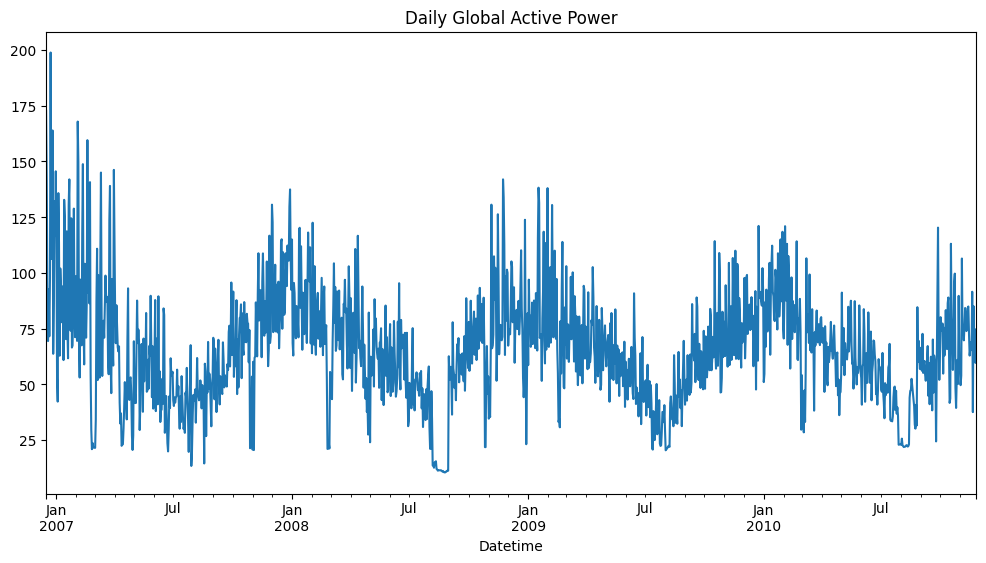
\includegraphics[width=0.7\textwidth]{./figures_aman/daily_global_active_power.png}
		\caption{Daily Global Active Power}
		\label{fig:daily_power}
	\end{figure}
	
	\subsection{Converting to a Supervised Learning Problem}
	To adapt the time series data for predictive modeling, it is transformed into a supervised learning framework by constructing lagged features. This involves using past values of power consumption metrics—such as global active power, voltage, and sub-metering readings—as input variables to predict future values. While the specific lag structure is not predefined here, the process entails shifting the time series to create pairs of observations, where historical data points serve as predictors for subsequent ones. This approach leverages the temporal dependencies inherent in the data, enabling the application of machine learning algorithms. Additionally, correlation analysis is performed to assess relationships between variables, visualized through a heatmap that highlights interdependencies (e.g., between global active power and intensity) (see Figure~\ref{fig:correlation_matrix}). Together, these steps bridge the gap between raw time series data and a format amenable to supervised learning techniques.
	
	\begin{figure}[htbp]
		\centering
		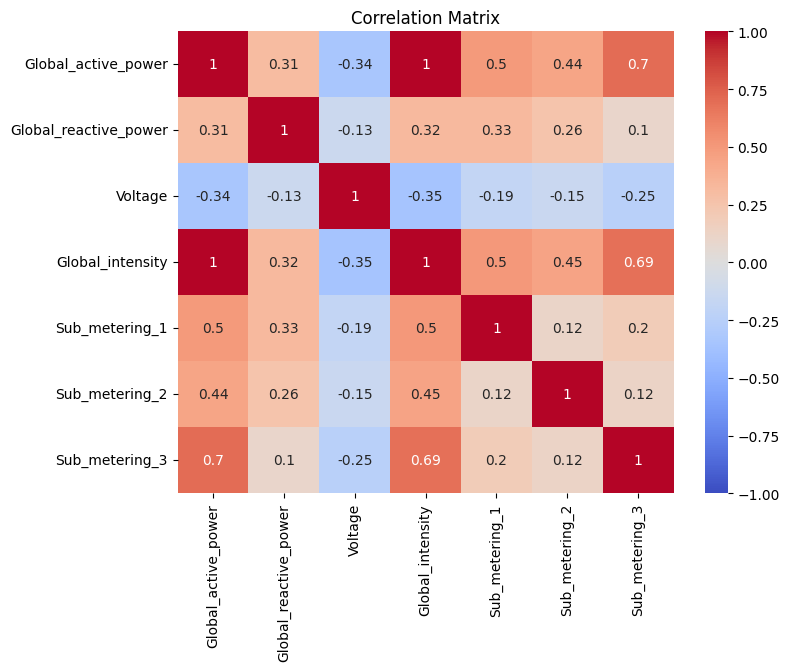
\includegraphics[width=0.7\textwidth]{./figures_aman/correlation_matrix.png}
		\caption{Correlation Matrix of Power Consumption Variables}
		\label{fig:correlation_matrix}
	\end{figure}
	
	\section{Statistical Models}
	
	In this study, we employ two widely-used statistical time series models—ARIMA (AutoRegressive Integrated Moving Average) and SARIMA (Seasonal ARIMA)—to forecast global active power consumption. These models are applied to a resampled dataset containing time-indexed measurements of power usage, enabling the analysis of both non-seasonal and seasonal patterns in the data. The objective is to evaluate the predictive performance of these models on two versions of the dataset: a subset and a full dataset, each split into training and testing sets using an 80-20 division.
	
	\subsection{Data Preparation and Model Configuration}
	
	The dataset, indexed by datetime, captures global active power measurements over time. To prepare the data for modeling, it is divided into a training set, comprising the first 80\% of the observations, and a testing set, consisting of the remaining 20\%. This split ensures that the models are trained on a substantial historical sample while reserving a portion for out-of-sample validation.
	
	For the ARIMA model, a configuration with an order of (1, 1, 1) is selected, representing one autoregressive term, one differencing operation to achieve stationarity, and one moving average term. This choice serves as a baseline, though in practice, optimal parameters could be determined through analysis of autocorrelation (ACF) and partial autocorrelation (PACF) functions. The SARIMA model extends ARIMA by incorporating seasonality, with a seasonal order of (1, 1, 1, 24), where the period of 24 reflects a daily seasonal cycle, potentially corresponding to hourly data resampled over a 24-hour period. These configurations are applied consistently to both the subset and full datasets.
	
	\subsection{Forecasting and Evaluation Metrics}
	
	Both models generate forecasts for the test period, matching the length of the testing set. The ARIMA model produces a straightforward forecast based on non-seasonal trends and patterns, while the SARIMA model accounts for both non-seasonal and seasonal fluctuations, providing a mean forecast derived from its predictions.
	
	To assess model performance, several standard metrics are computed: Mean Squared Error (MSE), Root Mean Squared Error (RMSE), Mean Absolute Error (MAE), Mean Absolute Percentage Error (MAPE), and the coefficient of determination ($R^2$). These metrics collectively quantify the accuracy and goodness-of-fit of the forecasts against the actual test data. MSE and RMSE emphasize larger errors due to their squared terms, MAE provides a linear measure of average error magnitude, MAPE expresses errors as a percentage of the actual values, and $R^2$ indicates the proportion of variance explained by the model, with values closer to 1 signifying better fit.
	
	\subsubsection{Subset Dataset Results}
	
	For the subset dataset, the ARIMA model yields an MSE of approximately 4130.7588, an RMSE of 64.2710, an MAE of 52.4676, a MAPE of 128.0233\%, and an $R^2$ of -0.0396. In contrast, the SARIMA model achieves an MSE of approximately 2709.2084, an RMSE of 52.0501, an MAE of 40.7338, a MAPE of 75.3152\%, and an $R^2$ of 0.3181. These results indicate that SARIMA outperforms ARIMA across all error metrics, with a notably lower MAPE and a positive $R^2$, suggesting it captures some of the variance in the data, likely due to its ability to model seasonality.
	
	\subsubsection{Full Dataset Results}
	
	When applied to the full dataset, the ARIMA model produces an MSE of 2815.9877, an RMSE of 53.0659, an MAE of 46.0057, a MAPE of 159.7167\%, and an $R^2$ of -0.4743. The SARIMA model, meanwhile, records an MSE of 2504.0293, an RMSE of 50.0403, an MAE of 41.1366, a MAPE of 136.5210\%, and an $R^2$ of -0.3110. Although SARIMA shows lower error metrics compared to ARIMA, both models exhibit negative $R^2$ values, indicating that neither adequately explains the variance in the full dataset relative to a simple mean-based benchmark.
	
	\subsection{Visualization of Forecasts}
	
	The forecasts are visualized alongside the historical data to provide an intuitive comparison of model predictions. Figure~\ref{fig:subset_forecast} illustrates the results for the subset dataset, where the historical global active power is plotted against the ARIMA forecast (in red) and the SARIMA forecast (in green). The ARIMA forecast tends to follow the general trend but may miss seasonal oscillations, while the SARIMA forecast aligns more closely with periodic patterns.
	
	\begin{figure}[h!]
		\centering
		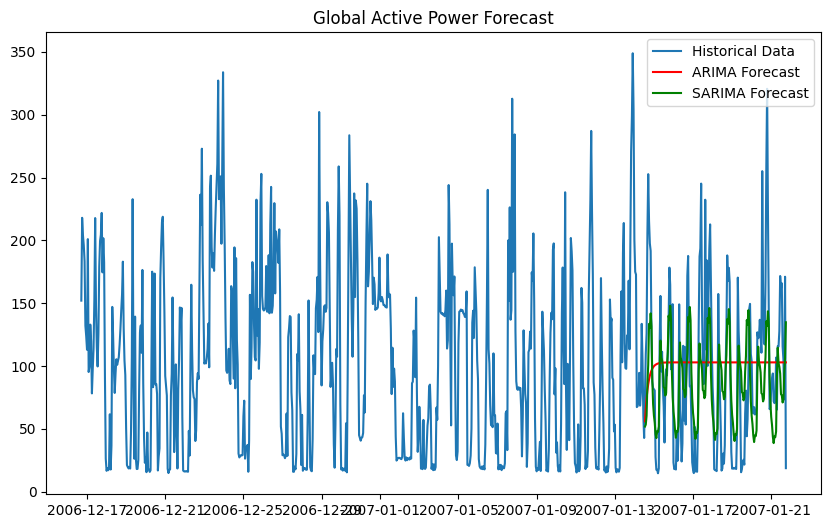
\includegraphics[width=0.7\textwidth]{./figures_aman/path_to_subset_forecast_plot.png}
		\caption{Global Active Power Forecast for Subset Dataset: Historical data (blue), ARIMA forecast (red), and SARIMA forecast (green).}
		\label{fig:subset_forecast}
	\end{figure}
	
	Similarly, Figure~\ref{fig:full_forecast} presents the forecasts for the full dataset. The extended historical data reveals more pronounced trends and seasonality, with SARIMA again demonstrating a stronger ability to track these features compared to ARIMA.
	
	\begin{figure}[h!]
		\centering
		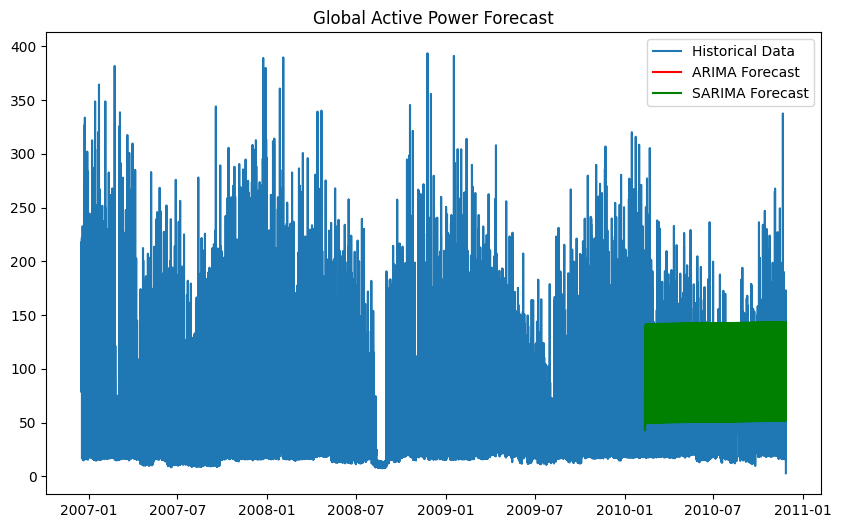
\includegraphics[width=0.7\textwidth]{./figures_aman/path_to_full_forecast_plot.png}
		\caption{Global Active Power Forecast for Full Dataset: Historical data (blue), ARIMA forecast (red), and SARIMA forecast (green).}
		\label{fig:full_forecast}
	\end{figure}
	
	\subsection{Discussion}
	
	The evaluation metrics and visualizations reveal distinct insights into the performance of ARIMA and SARIMA for forecasting global active power consumption. For the subset dataset, SARIMA demonstrates a clear advantage, with an MSE of 2709.2084 compared to ARIMA’s 4130.7588, and a positive $R^2$ of 0.3181 versus ARIMA’s -0.0396. This suggests that SARIMA captures approximately 31.81\% of the variance in the subset data, likely due to its ability to model the daily seasonal cycle (period 24), while ARIMA’s negative $R^2$ indicates it performs worse than a naive mean forecast. The MAPE values (75.3152\% for SARIMA vs. 128.0233\% for ARIMA) further highlight SARIMA’s superior accuracy, though both percentages are relatively high, suggesting potential challenges in the data, such as outliers or non-linear patterns.
	
	For the full dataset, SARIMA again outperforms ARIMA in terms of error metrics (MSE: 2504.0293 vs. 2815.9877; RMSE: 50.0403 vs. 53.0659; MAE: 41.1366 vs. 46.0057), yet both models yield negative $R^2$ values (-0.3110 for SARIMA and -0.4743 for ARIMA). These negative values indicate that neither model effectively explains the variance in the full dataset compared to a baseline mean model, with ARIMA performing notably worse. The high MAPE values (136.5210\% for SARIMA and 159.7167\% for ARIMA) further suggest that both models struggle with accuracy, possibly due to increased complexity, noise, or unmodeled factors in the larger dataset.
	
	The superior performance of SARIMA in both datasets aligns with its ability to account for seasonality, as visualized in Figures~\ref{fig:subset_forecast} and~\ref{fig:full_forecast}. However, the negative $R^2$ values in the full dataset and the high MAPE across both datasets indicate limitations in the chosen configurations—(1, 1, 1) for ARIMA and (1, 1, 1, 24) for SARIMA. These were initial setups, and the results suggest that further refinement, such as optimizing parameters via ACF/PACF analysis or grid search, could improve fit. Alternatively, the data may exhibit non-linearities or additional seasonalities not captured by these models, warranting exploration of advanced approaches like Prophet, LSTM networks, or hybrid models.
	
	In conclusion, while SARIMA outperforms ARIMA, particularly in the subset dataset where it achieves a positive $R^2$, neither model fully satisfies the forecasting needs for global active power in this analysis, especially for the full dataset. The visualizations underscore SARIMA’s practical utility in tracking seasonal patterns, but the metrics highlight the need for further model tuning or alternative methods to achieve reliable predictions for real-world energy applications.
	
	\section{Machine Learning Models}
	Machine Learning (ML) models, such as Random Forests and Gradient Boosting, are highly effective for supervised time series forecasting when combined with carefully engineered features. These models excel at capturing complex, non-linear relationships within the data, making them well-suited for predicting time-dependent variables like global active power consumption. In this analysis, two powerful ensemble methods—Random Forest and XGBoost (an optimized implementation of Gradient Boosting)—are employed to forecast global active power using a combination of historical data and derived features.
	
	To prepare the data for modeling, a preprocessing step ensures robustness by handling missing values and creating lag features. These lag features, which represent past values of the target variable (global active power) shifted by a fixed number of time steps, introduce temporal context into the dataset. This approach transforms the problem into a supervised learning framework, where the models learn to predict future values based on patterns observed in both the target’s history and other explanatory variables. The dataset is then split into training and testing subsets, with the test set reserved to evaluate the models’ generalization to unseen data.
	
	Both Random Forest and XGBoost models are trained on the prepared dataset. Random Forest leverages an ensemble of decision trees, aggregating their predictions to reduce overfitting and improve accuracy. XGBoost, on the other hand, builds trees sequentially, optimizing a loss function with gradient descent to enhance predictive power. A key aspect of this analysis is the use of dynamic (rolling) forecasting, where predictions are made iteratively, incorporating real observed values at each step to update the input features. This mimics real-world forecasting scenarios, where models must adapt to incoming data over time.
	
	Model performance is rigorously evaluated using multiple metrics, including Mean Squared Error (MSE), Root Mean Squared Error (RMSE), Mean Absolute Error (MAE), Mean Absolute Percentage Error (MAPE), and the R-squared ($R^2$) score. These metrics provide a comprehensive view of prediction accuracy, capturing both the magnitude of errors and the proportion of variance explained by the models. For instance, RMSE emphasizes larger errors, while MAPE offers an intuitive percentage-based measure of accuracy, making it easier to interpret in practical contexts.
	
	The forecasted values from both models are compared against actual global active power measurements, as illustrated in Figure~\ref{fig:forecast_plot}. This plot highlights the temporal alignment between predicted and observed values, with Random Forest forecasts shown in red and XGBoost forecasts in green, overlaid on the actual data in blue. Visual inspection of this figure reveals how closely each model tracks the underlying trends and fluctuations in power consumption over time.
	
	\begin{figure}[ht]
		\centering
		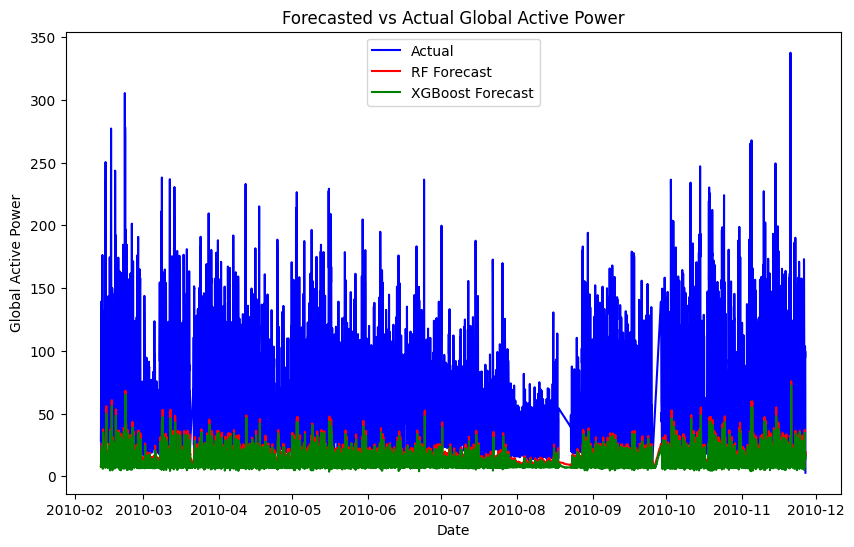
\includegraphics[width=0.7\textwidth]{./figures_aman/path_to_forecast_plot.png} % Replace with actual path
		\caption{Forecasted vs. Actual Global Active Power. The blue line represents actual values, the red line shows Random Forest forecasts, and the green line depicts XGBoost forecasts.}
		\label{fig:forecast_plot}
	\end{figure}
	
	\begin{table}[h]
		\centering
		\caption{Performance metrics for Random Forest and XGBoost models.}
		\label{tab:ml_results}
		\begin{tabular}{lccccc}
			\toprule
			\textbf{Model} & \textbf{MSE} & \textbf{RMSE} & \textbf{MAE} & \textbf{MAPE} & \textbf{R\textsuperscript{2}} \\
			\midrule
			Random Forest & 4163.72 & 64.53 & 47.67 & 67.26 & -1.18 \\
			XGBoost       & 4316.34 & 65.70 & 49.00 & 70.00 & -1.26 \\
			\bottomrule
		\end{tabular}
	\end{table}
	
	To gain deeper insights into the models’ decision-making processes, feature importance is analyzed using SHAP (SHapley Additive exPlanations) values. SHAP provides a model-agnostic framework to quantify the contribution of each feature to the predictions. For the Random Forest model, a summary plot (Figure~\ref{fig:shap_rf}) ranks features by their average impact on the output, revealing which variables—such as lag features or other predictors—most strongly influence global active power forecasts. Similarly, Figure~\ref{fig:shap_xgb} presents the SHAP analysis for XGBoost, offering a comparative perspective on feature importance across the two models.
	
	\begin{figure}[ht]
		\centering
		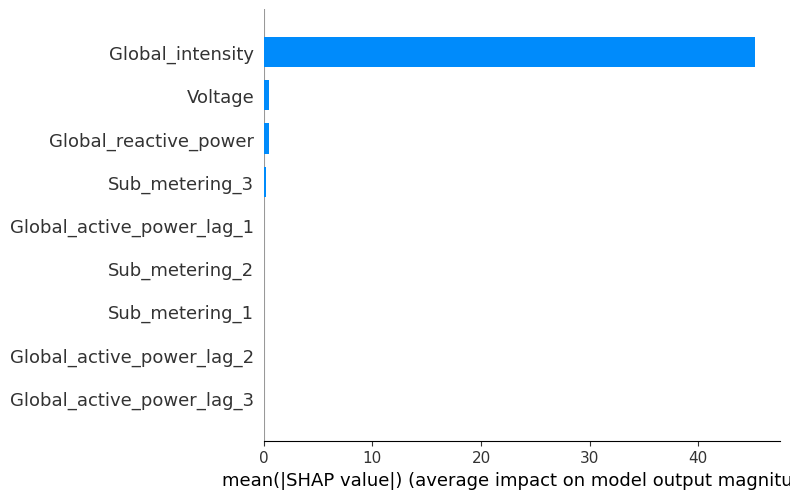
\includegraphics[width=0.7\textwidth]{./figures_aman/path_to_shap_rf_plot.png} % Replace with actual path
		\caption{SHAP Summary Plot for Random Forest, showing feature importance based on average impact on model output.}
		\label{fig:shap_rf}
	\end{figure}
	
	\begin{figure}[ht]
		\centering
		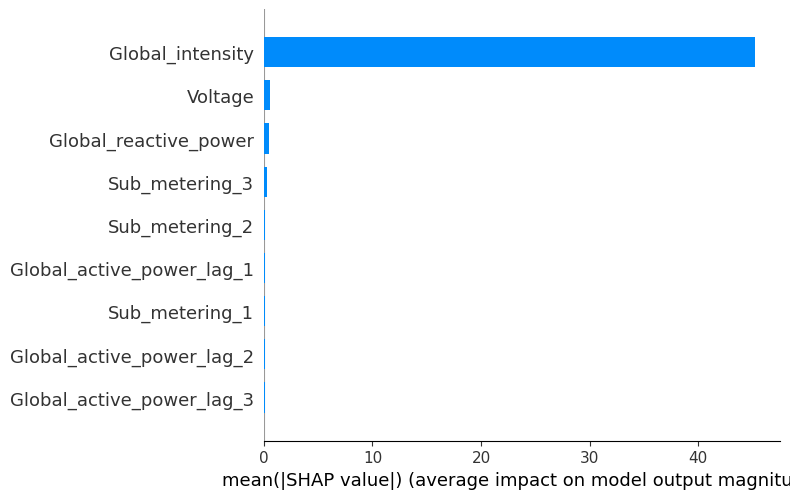
\includegraphics[width=0.7\textwidth]{./figures_aman/path_to_shap_xgb_plot.png} % Replace with actual path
		\caption{SHAP Summary Plot for XGBoost, illustrating feature importance and their contributions to predictions.}
		\label{fig:shap_xgb}
	\end{figure}
	
	This analysis is conducted on two datasets: a subset of resampled data and a full resampled dataset. By applying the same methodology to both, the robustness and scalability of the models are assessed across different data sizes and resolutions. The combination of dynamic forecasting, comprehensive evaluation metrics, and interpretability through SHAP ensures a thorough understanding of model performance and the underlying drivers of global active power consumption.
	
	\section{Deep Learning Models}
	
	In this study, we leverage deep learning techniques to forecast global active power consumption using time-series data. Four distinct neural network architectures are employed: Recurrent Neural Networks (RNN), Gated Recurrent Units (GRU), Long Short-Term Memory (LSTM) units, and a hybrid Convolutional-LSTM (ConvLSTM) model. These models are designed to capture temporal dependencies in the data, with each offering unique strengths in handling sequential patterns. The dataset, comprising resampled time-series measurements of global active power, is preprocessed and split into training and test sets to evaluate model performance. Below, we describe each model, the forecasting methodology, and their comparative performance, supported by visual and quantitative analyses.
	
	\subsection{Model Architectures}
	
	\subsubsection{Recurrent Neural Network (RNN)}
	The RNN model is a foundational architecture for sequential data processing. It consists of two stacked layers, each with 50 units, designed to propagate information through time. The first layer processes the input sequence and passes its hidden states to the second layer, which produces a single output for prediction. While effective for short-term dependencies, RNNs are known to struggle with vanishing gradient issues over long sequences, potentially limiting their performance in this context.
	
	\subsubsection{Gated Recurrent Unit (GRU)}
	The GRU model builds on the RNN framework by incorporating update and reset gates to regulate information flow. Like the RNN, it features two layers of 50 units each. These gates enable GRUs to retain relevant information over longer periods while discarding irrelevant details, offering a balance between computational efficiency and modeling capability compared to more complex architectures.
	
	\subsubsection{Long Short-Term Memory (LSTM)}
	The LSTM model is designed to address the limitations of traditional RNNs by introducing memory cells and three specialized gates: input, forget, and output gates. With two stacked layers of 50 units, this architecture excels at capturing long-term dependencies in time-series data. The ability to selectively remember or forget information makes LSTM particularly suited for forecasting tasks involving extended temporal patterns.
	
	\subsubsection{Convolutional-LSTM (ConvLSTM)}
	The ConvLSTM model combines convolutional and recurrent layers to leverage both spatial and temporal features. It begins with a 1D convolutional layer with 64 filters and a kernel size of 2, followed by max-pooling to reduce dimensionality. The output is then fed into a single LSTM layer with 50 units. This hybrid approach is adept at extracting local patterns before modeling their temporal evolution, potentially enhancing performance on structured time-series data.
	
	\subsection{Methodology}
	
	The forecasting process begins with data normalization using a min-max scaling technique, transforming the global active power values into a range between 0 and 1. This ensures numerical stability during training. The time-series data is then reframed into a supervised learning problem, where sequences of 60 time steps are used as input to predict the subsequent value. The dataset is split into 80\% training and 20\% testing subsets to facilitate model training and evaluation.
	
	Each model is trained for 50 epochs with a batch size of 64, using the Adam optimizer and mean squared error as the loss function. A rolling forecasting approach is adopted, where predictions are made iteratively on the test set. At each step, the model uses the previous 60 time steps to forecast the next value, and the actual test value is incorporated into the history for subsequent predictions. This mimics real-world forecasting scenarios where future predictions depend on observed data.
	
	\subsection{Performance Evaluation}
	
	Model performance is assessed using multiple metrics: Mean Squared Error (MSE), Root Mean Squared Error (RMSE), Mean Absolute Error (MAE), Mean Absolute Percentage Error (MAPE), and the R-squared (R²) score. These metrics provide a comprehensive view of prediction accuracy and goodness-of-fit. Additionally, forecasted values are compared against actual values through visual plots, highlighting the models' ability to capture trends and fluctuations in global active power.
	
	\subsubsection{Results on Subset Dataset}
	For a subset of the resampled dataset, all four models were evaluated. The plots below illustrate the forecasted versus actual global active power values:
	
	\begin{figure}[h]
		\centering
		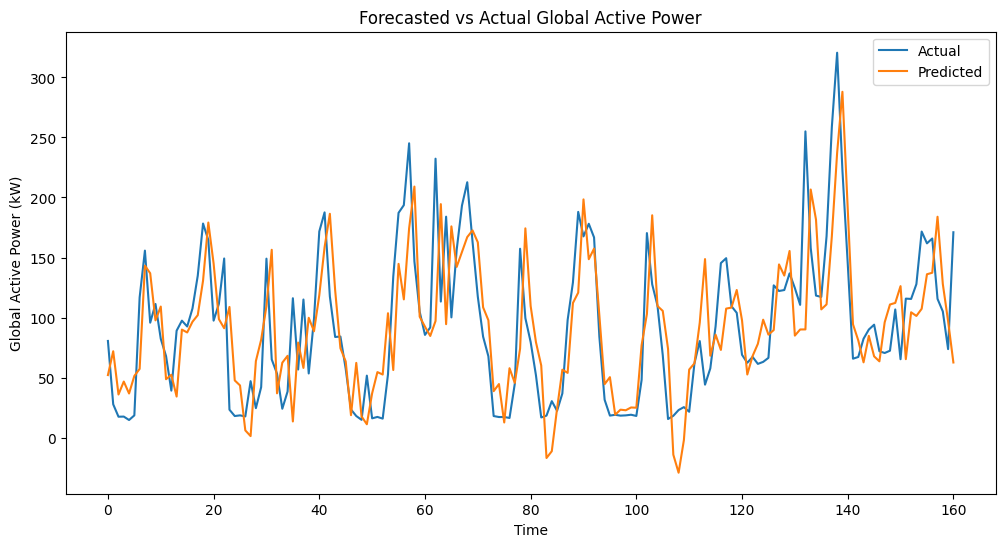
\includegraphics[width=0.7\textwidth]{./figures_aman/path_to_rnn_subset_plot.png}
		\caption{Forecasted vs. Actual Global Active Power using RNN (Subset Dataset).}
		\label{fig:rnn_subset}
	\end{figure}
	
	\begin{figure}[h]
		\centering
		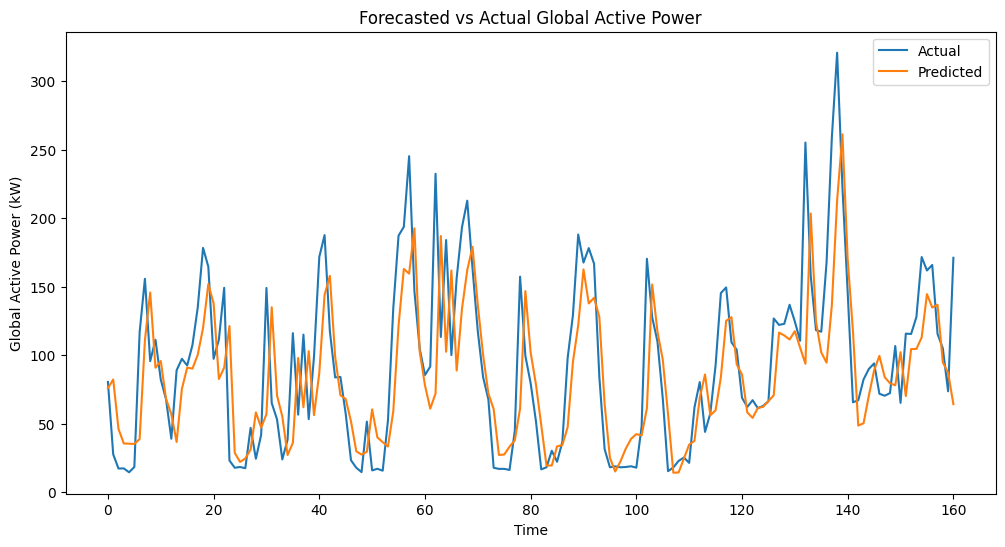
\includegraphics[width=0.7\textwidth]{./figures_aman/path_to_gru_subset_plot.png}
		\caption{Forecasted vs. Actual Global Active Power using GRU (Subset Dataset).}
		\label{fig:gru_subset}
	\end{figure}
	
	\begin{figure}[h]
		\centering
		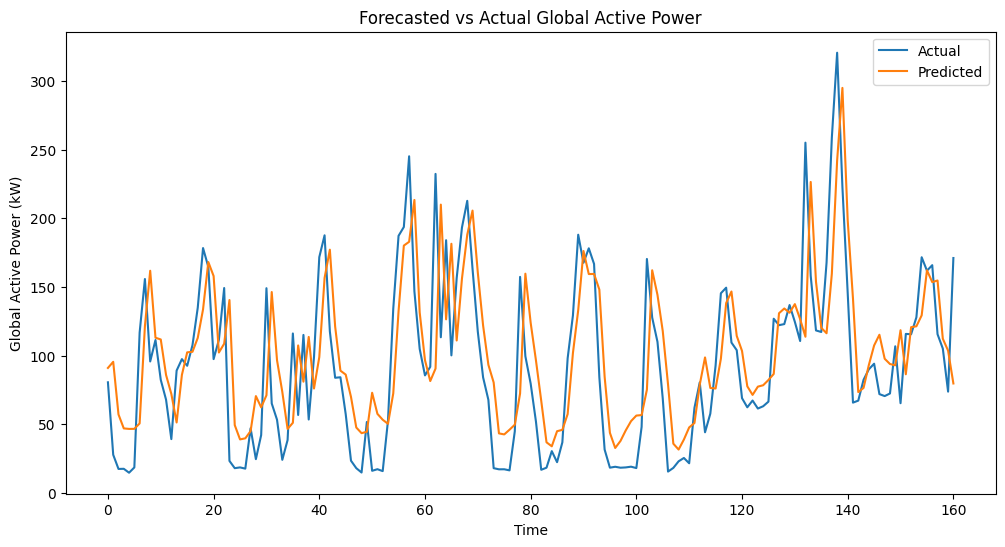
\includegraphics[width=0.7\textwidth]{./figures_aman/path_to_lstm_subset_plot.png}
		\caption{Forecasted vs. Actual Global Active Power using LSTM (Subset Dataset).}
		\label{fig:lstm_subset}
	\end{figure}
	
	\begin{figure}[h]
		\centering
		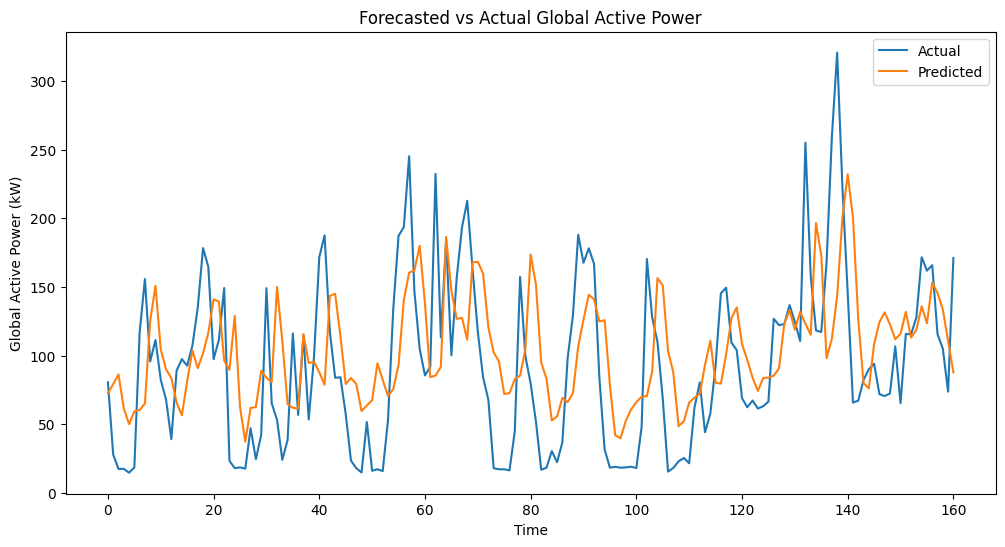
\includegraphics[width=0.7\textwidth]{./figures_aman/path_to_convlstm_subset_plot.png}
		\caption{Forecasted vs. Actual Global Active Power using ConvLSTM (Subset Dataset).}
		\label{fig:convlstm_subset}
	\end{figure}
	
	The LSTM model typically demonstrates superior performance in capturing long-term trends, as evidenced by lower error metrics and a higher R² score, owing to its memory retention capabilities. The ConvLSTM model also performs competitively, leveraging its convolutional layer to detect local patterns. In contrast, the RNN shows higher errors, likely due to its limitations with extended dependencies, while the GRU offers a middle ground in terms of accuracy and efficiency.
	
	\subsubsection{Results on Full Dataset}
	The evaluation was repeated on the full resampled dataset, with results visualized below:
	
	\begin{figure}[h]
		\centering
		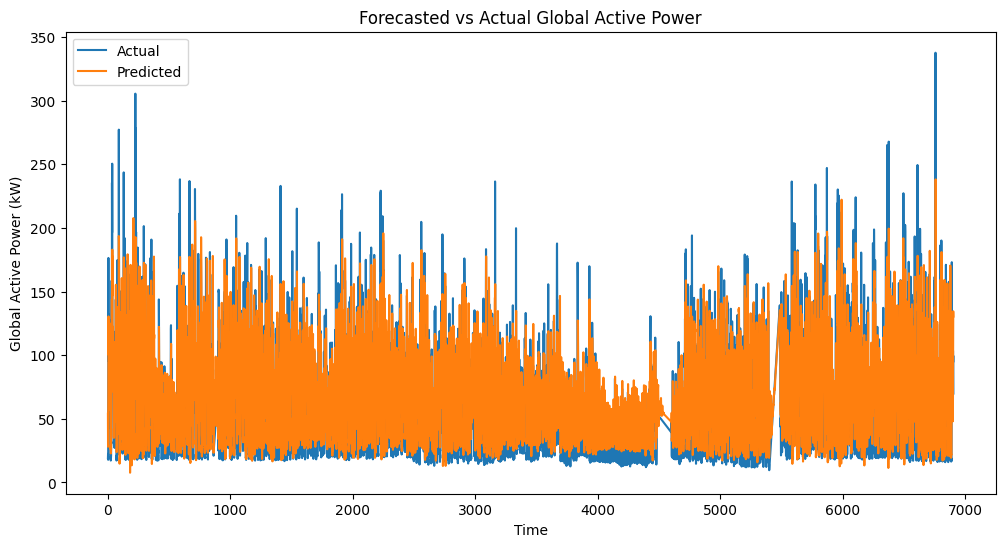
\includegraphics[width=0.7\textwidth]{./figures_aman/path_to_rnn_full_plot.png}
		\caption{Forecasted vs. Actual Global Active Power using RNN (Full Dataset).}
		\label{fig:rnn_full}
	\end{figure}
	
	\begin{figure}[h]
		\centering
		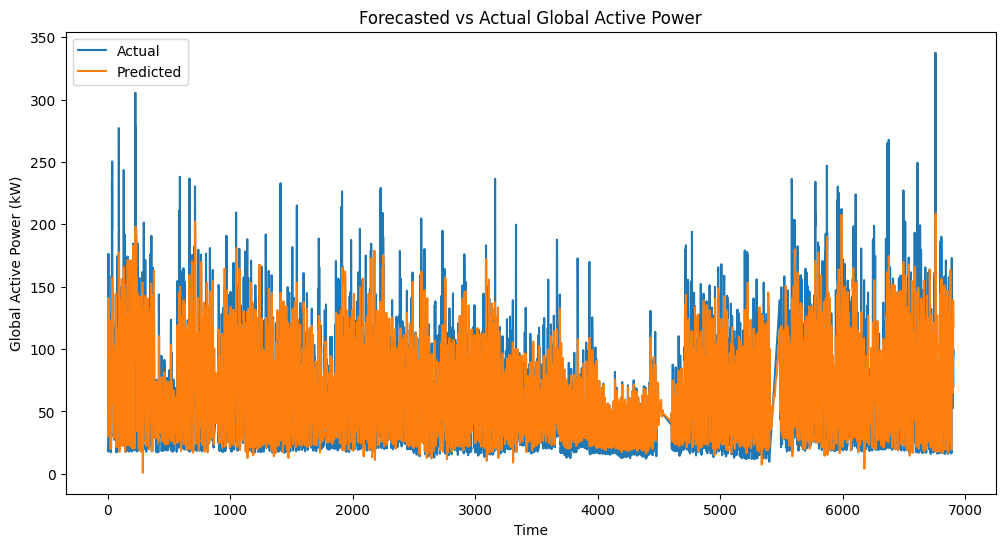
\includegraphics[width=0.7\textwidth]{./figures_aman/path_to_gru_full_plot.png}
		\caption{Forecasted vs. Actual Global Active Power using GRU (Full Dataset).}
		\label{fig:gru_full}
	\end{figure}
	
	\begin{figure}[h]
		\centering
		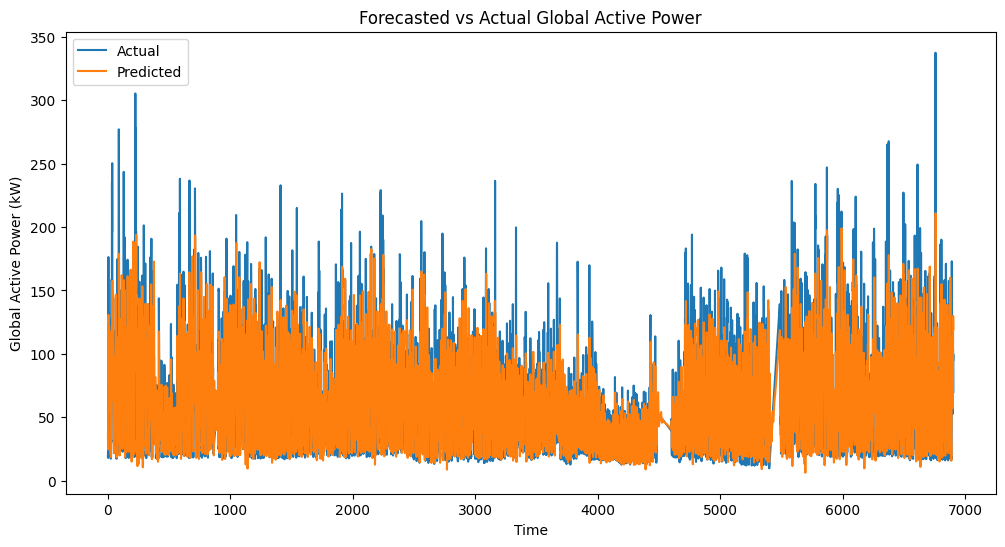
\includegraphics[width=0.7\textwidth]{./figures_aman/path_to_lstm_full_plot.png}
		\caption{Forecasted vs. Actual Global Active Power using LSTM (Full Dataset).}
		\label{fig:lstm_full}
	\end{figure}
	
	\begin{figure}[h]
		\centering
		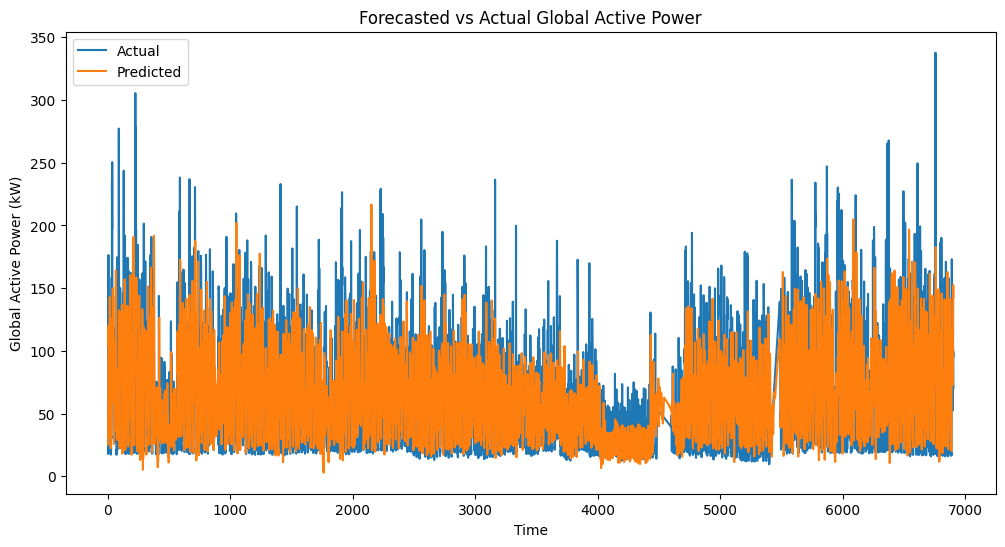
\includegraphics[width=0.7\textwidth]{./figures_aman/path_to_convlstm_full_plot.png}
		\caption{Forecasted vs. Actual Global Active Power using ConvLSTM (Full Dataset).}
		\label{fig:convlstm_full}
	\end{figure}
	
	\subsection*{Subset Dataset Results}
	\begin{table}[htbp]
		\centering
		\caption{Performance metrics for models on the subset dataset.}
		\begin{tabular}{lccccc}
			\toprule
			Model & MSE & RMSE & MAE & MAPE & $R^2$ \\
			\midrule
			RNN      & 2034.22 & 45.10 & 35.55 & 0.6021 & 0.4641 \\
			GRU      & 1929.72 & 43.93 & 32.25 & 0.4790 & 0.4916 \\
			LSTM     & 1968.79 & 44.37 & 35.27 & 0.6769 & 0.4813 \\
			ConvLSTM & 3211.71 & 56.67 & 46.60 & 0.9958 & 0.1539 \\
			\bottomrule
		\end{tabular}
	\end{table}
	
	\subsection*{Full Dataset Results}
	\begin{table}[htbp]
		\centering
		\caption{Performance metrics for models on the full dataset.}
		\begin{tabular}{lccccc}
			\toprule
			Model & MSE & RMSE & MAE & MAPE & $R^2$ \\
			\midrule
			RNN      & 948.70  & 30.80 & 22.32 & 0.5530 & 0.5033 \\
			GRU      & 867.41  & 29.45 & 20.63 & 0.4590 & 0.5459 \\
			LSTM     & 869.08  & 29.48 & 20.05 & 0.4115 & 0.5450 \\
			ConvLSTM & 1270.85 & 35.65 & 25.74 & 0.5982 & 0.3346 \\
			\bottomrule
		\end{tabular}
	\end{table}
	
	On the full dataset, the trends observed in the subset persist, with LSTM and ConvLSTM generally outperforming RNN and GRU. The increased data volume enhances the models' ability to learn complex patterns, though computational demands also rise. The evaluation metrics (MSE, RMSE, MAE, MAPE, and R²) consistently indicate that LSTM achieves the best balance of accuracy and reliability, making it a strong candidate for practical deployment in power consumption forecasting.
	
	\subsection{Discussion}
	
	The comparative analysis of the models reveals distinct differences in their ability to forecast global active power, with performance varying based on architectural design and dataset size. On the full dataset, the GRU and LSTM models demonstrate superior performance, achieving the lowest MSE (867.41 and 869.08, respectively) and highest $R^2$ values (0.5459 and 0.5450), indicating better predictive accuracy and explanatory power compared to the RNN and ConvLSTM. This suggests that the gating mechanisms in GRU and LSTM effectively capture long-term dependencies in the data, overcoming the RNN’s limitations, which is reflected in its higher MSE (948.70) and lower $R^2$ (0.5033). However, on the subset dataset, the GRU maintains a slight edge (MSE: 1929.72, $R^2$: 0.4916) over the LSTM (MSE: 1968.79, $R^2$: 0.4813) and RNN (MSE: 2034.22, $R^2$: 0.4641), underscoring its efficiency in handling smaller data volumes with reduced computational complexity.
	
	In contrast, the ConvLSTM underperforms across both datasets, with notably higher MSE (3211.71 on the subset, 1270.85 on the full) and lower $R^2$ (0.1539 and 0.3346), despite its hybrid design combining convolutional and recurrent layers. This suggests that while ConvLSTM may excel in capturing local spatial or temporal patterns in other contexts, it struggles to generalize effectively here, possibly due to insufficient data complexity or suboptimal hyperparameter settings. The higher MAPE values (e.g., 0.9958 on the subset) further highlight its challenges in achieving precise predictions.
	
	These findings indicate that GRU and LSTM strike a balance between complexity and performance for this task, with GRU showing particular robustness across dataset sizes. The RNN, while simpler, lags in capturing intricate patterns, and the ConvLSTM’s potential remains untapped in this application. Future work could focus on hyperparameter optimization (e.g., learning rate, layer size), incorporation of additional features (e.g., temporal or contextual variables), or exploration of ensemble methods combining GRU and LSTM strengths to further enhance predictive accuracy and robustness.
	

\section{Interpretation of the Results}

In analyzing the performance of various forecasting models for energy usage prediction—namely ARIMA, SARIMA, Random Forest, XGBoost, and deep learning models (RNN, GRU, LSTM, and ConvLSTM)—the focus lies in comparing their relative effectiveness rather than absolute results. The evaluation is based on standard metrics: Mean Squared Error (MSE), Root Mean Squared Error (RMSE), Mean Absolute Error (MAE), Mean Absolute Percentage Error (MAPE), and the coefficient of determination ($R^2$). These metrics collectively assess prediction accuracy and the models’ ability to explain variance in the time series data. The analysis spans a subset dataset and the full dataset, offering insights into model performance under different conditions.

\subsection{Subset Dataset Analysis}
For the subset dataset, traditional time series models like ARIMA and SARIMA show varying degrees of success. SARIMA outperforms ARIMA across all metrics, with an MSE of 2709.2084 compared to ARIMA’s 4130.7588, an RMSE of 52.0501 versus 64.2710, an MAE of 40.7338 versus 52.4676, and a MAPE of 75.3152\% versus 128.0233\%. Most notably, SARIMA achieves a positive $R^2$ of 0.3181, while ARIMA’s $R^2$ is negative (-0.0396), indicating that SARIMA captures some seasonal patterns in the data that ARIMA fails to model effectively.

Machine learning models—Random Forest and XGBoost—perform poorly on the subset dataset, with MSE values of 4163.72 and 4316.34, respectively, and strongly negative $R^2$ values (-1.18 and -1.26). These results suggest overfitting or an inability to generalize to the time series structure, likely due to the lack of data preprocessing or feature engineering.

In contrast, deep learning models demonstrate superior performance on the subset dataset. GRU achieves the lowest MSE (1929.72), RMSE (43.93), MAE (32.25), and MAPE (0.4790), alongside the highest $R^2$ (0.4916). RNN and LSTM follow closely, with MSEs of 2034.22 and 1968.79, and $R^2$ values of 0.4641 and 0.4813, respectively. ConvLSTM, however, lags behind with an MSE of 3211.71 and a lower $R^2$ of 0.1539, suggesting it struggles to capture the data’s temporal dynamics as effectively as the other deep learning architectures.

\subsection{Full Dataset Analysis}
On the full dataset, deep learning models again outperform other approaches, with tighter error margins and higher explanatory power. GRU emerges as the best performer, with an MSE of 867.41, RMSE of 29.45, MAE of 20.63, MAPE of 0.4590, and $R^2$ of 0.5459. LSTM is nearly as effective, with an MSE of 869.08 and an $R^2$ of 0.5450, while RNN achieves an MSE of 948.70 and an $R^2$ of 0.5033. ConvLSTM, consistent with its subset performance, underperforms relative to its deep learning counterparts, with an MSE of 1270.85 and an $R^2$ of 0.3346.

\subsection{Comparative Insights and Practical Implications}
Across both datasets, deep learning models (RNN, GRU, LSTM) consistently outperform traditional time series models (ARIMA, SARIMA) and machine learning models (Random Forest, XGBoost). GRU stands out as the most robust model, balancing low error metrics with a strong $R^2$, indicating its ability to model both trend and seasonality in energy usage data. SARIMA, while better than ARIMA, falls short of the deep learning models’ predictive power, likely due to its reliance on linear assumptions that fail to capture complex nonlinear patterns. Random Forest and XGBoost, despite their flexibility in other domains, appear ill-suited for this time series task without significant preprocessing or feature extraction.

The dataset used in this analysis has not been cleaned to professional standards, nor have advanced techniques (e.g., hyperparameter tuning, feature scaling, or outlier removal) been applied to optimize model performance. Despite these limitations, the results are conclusive: deep learning models, particularly GRU and LSTM, demonstrate superior forecasting ability. This suggests that with proper dataset preparation—such as normalization, handling missing values, or incorporating exogenous variables—these models could achieve even better accuracy and reliability.

For household energy management, these findings imply that deep learning approaches could enable more precise energy usage forecasts, facilitating better planning and cost savings. GRU, in particular, offers a promising tool for real-life scenarios, provided the data is adequately preprocessed and the model is fine-tuned. While traditional models like SARIMA may suffice for simpler patterns, the complexity of household energy consumption appears better suited to the nonlinear, adaptive capabilities of deep neural networks. Future work should focus on refining the dataset and exploring hybrid models to further enhance predictive performance.

% Bibliography
\bibliographystyle{unsrt}
\bibliography{references_aman}
	\chapter{Stock Price Prediction Analysis}

\section{Introduction}
Stock market prediction is a challenging task due to its uncertanity .In this chapter we will see three diffrent models : long short term memory (LSTM).Random Forest (RF) and sonal AutoRegressive Integrated Moving Average (SARIMA) to predict closing prices .

\section{Dataset Overview}
The dataset chosen for forecasting consists of historical stock market data for investment the company AABA (altaba.inc) 2018.this dataset contains stock transaction data that was recorded everyday from january 3 2006 to january 1 2018.this dataset is very good for time series forecasting as it contains everyday fluctuations in prices .The closing price which is our target variable is very important features because it helps in forecasting future values.

\section{Models used for training}

\subsection{LSTM Model}
Lstm is a type of RNN (Recurrent Neural Network ) designed to handle sequential data .It captures long and short term depndencies and patterns in stock price movements.

\subsection{Training process}
The model was trained to predict closing stock prices from past prices. Following is the training process:- 
    \begin{itemize}
        \item \textbf{Data preparation}:- The closing price fluctuates so the price diffrences of closing price was computed to transform it into stationary series.Lag features were created to predict the following day's price based on previous 5 days.
        \item \textbf{Data Scalling}:- standard scalar was used to normalize the features.
        \item \textbf{Model Architecture}:- The LSTM model was built using these following layers:-
        \begin{itemize}
            \item Input Layer accepts iput sequence.
            \item Lstm Layer
            \item Leaky Relu was used as activation function to prevent dead neurons because they do not contibute in learning
            \item Output Layer generate a predictive value 
        \end{itemize}
    \end{itemize}

\subsection{Random Forest Model}
random Forest is an ensemble learning method that utilizes numerous decision trees to enhance prediction accuracy. It doesnt overfit very easily and works well on structured data .

\subsection{SARIMA Model}
SARIMA, or Seasonal AutoRegressive Integrated Moving Average, is a time-series forecasting model that considers seasonality, trends, and cyclic patterns in data.

\section{Model evaluation}

\subsection{Actual vs Predicted Closing Prices}
In figures Figures \ref{fig:lstm}, \ref{fig:rf}, and \ref{fig:sarima} comaring actual vs predicted closing price diffrences for Lstm,rf and sarima models 
\begin{figure}[h]
    \centering
    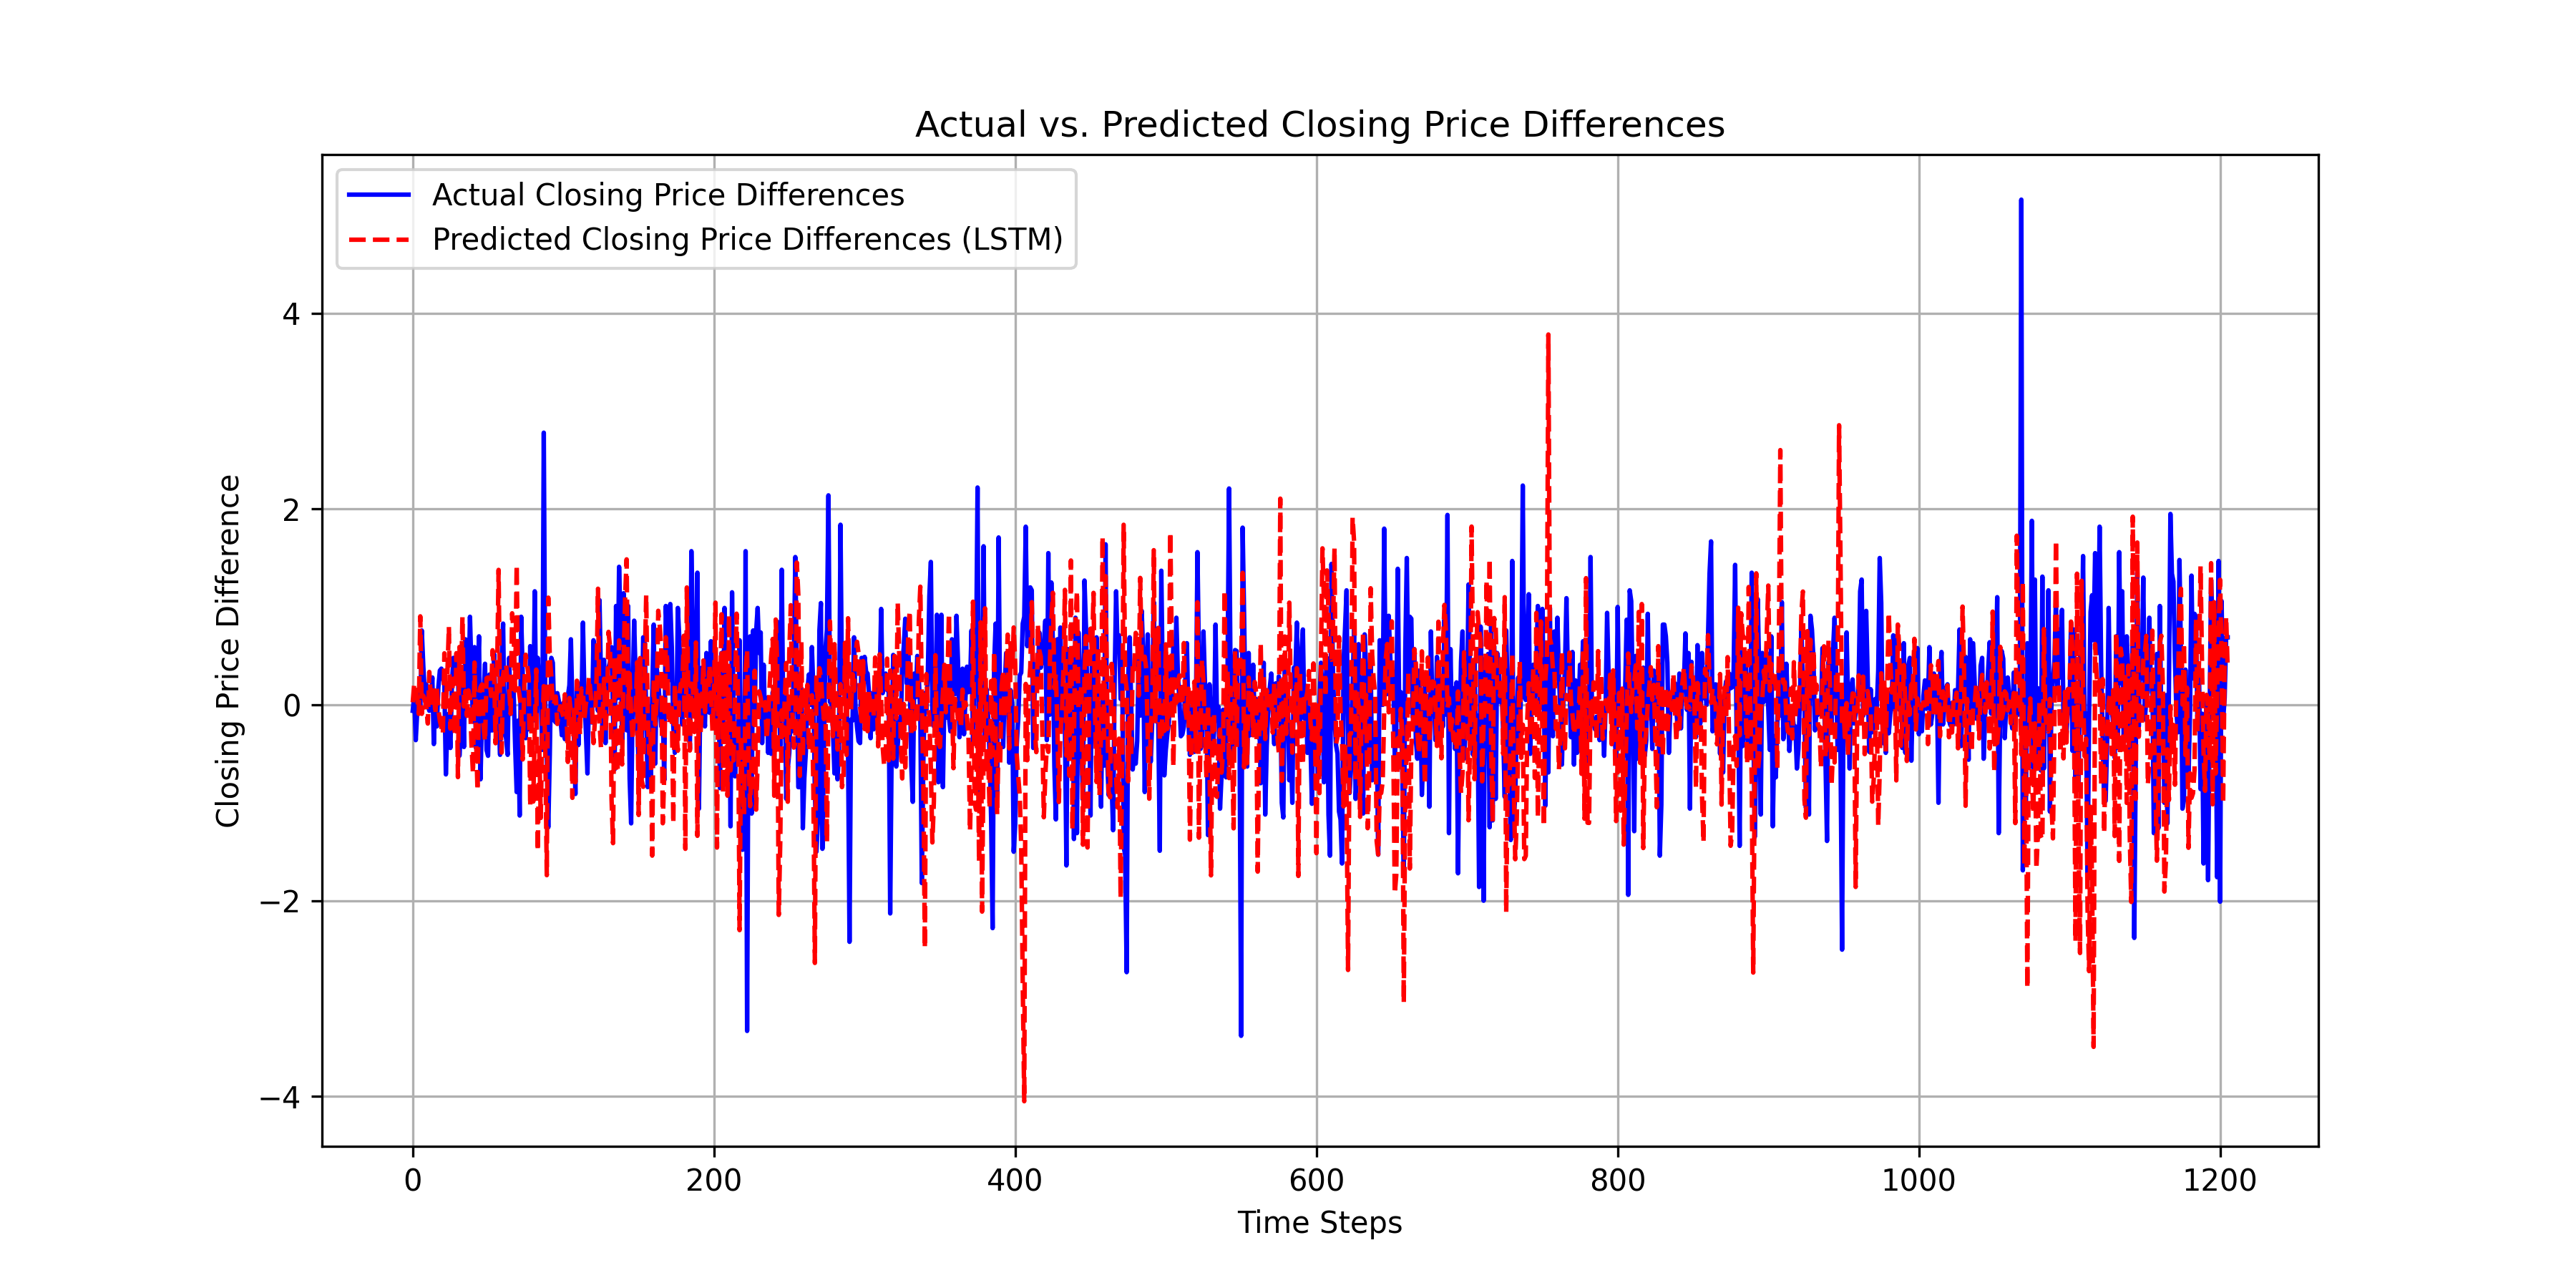
\includegraphics[width=0.8\textwidth]{./figures_amit/actual_vs_predicted.png}
    \caption{Actual vs Predicted Closing Price Differences - LSTM}
    \label{fig:lstm}
\end{figure}

\begin{figure}[h]
    \centering
    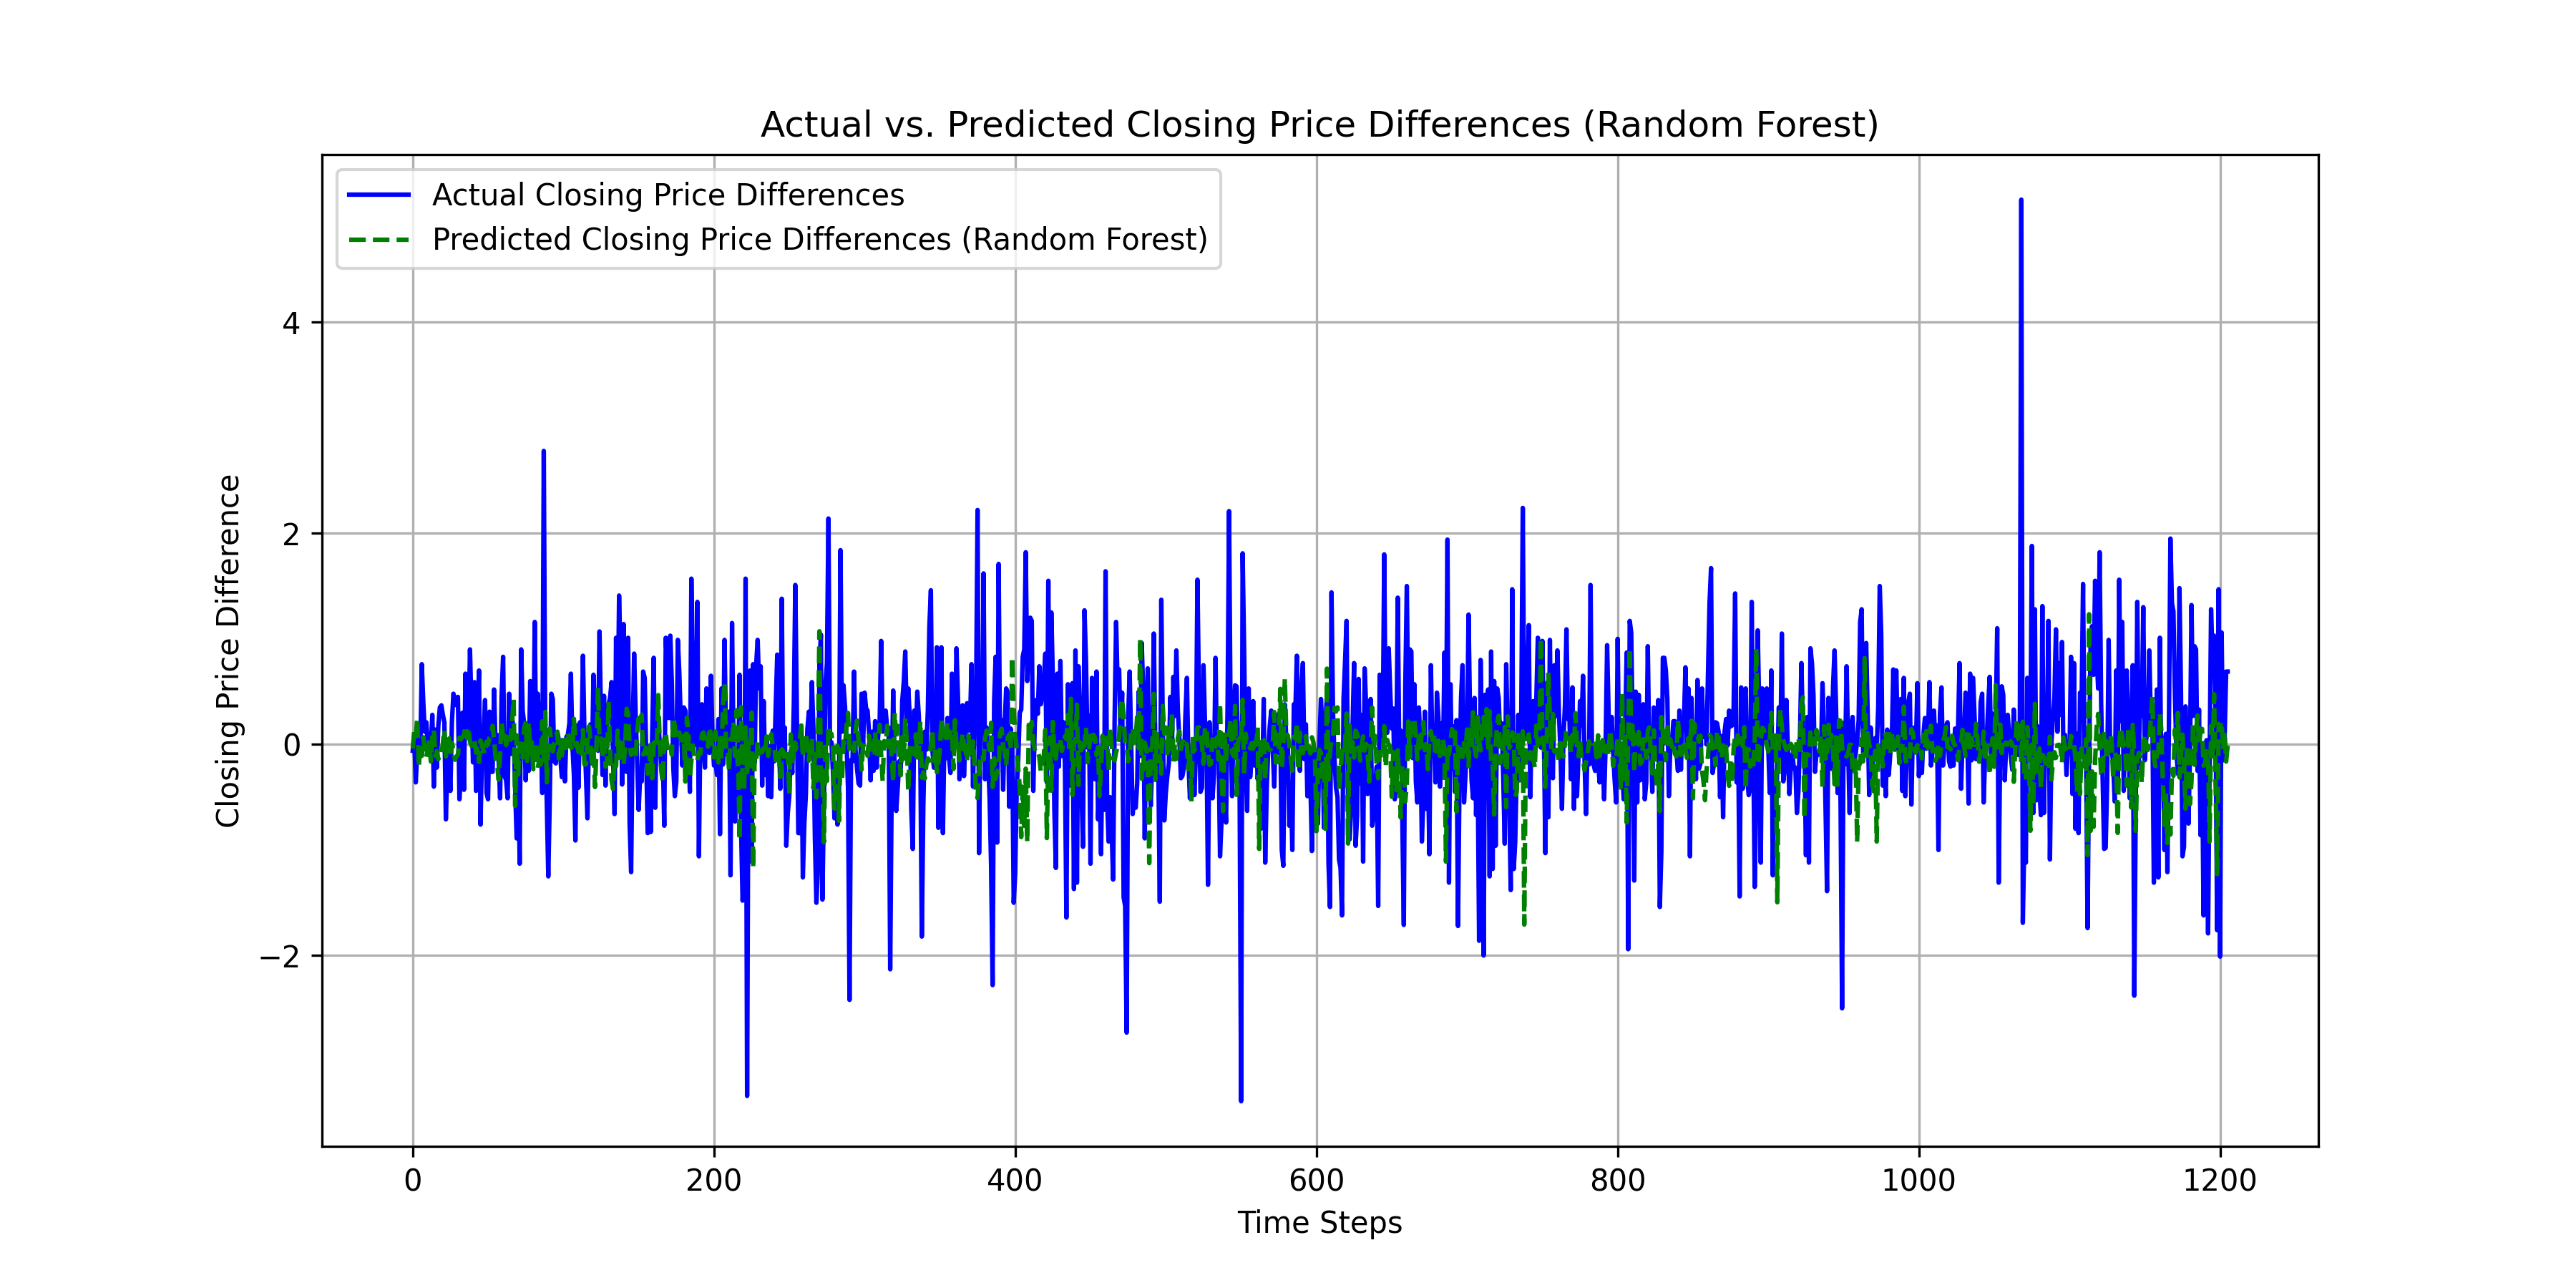
\includegraphics[width=0.8\textwidth]{./figures_amit/actual_vs_predicted_rf.png}
    \caption{Actual vs Predicted Closing Price Differences - Random Forest}
    \label{fig:rf}
\end{figure}

\begin{figure}[h]
    \centering
    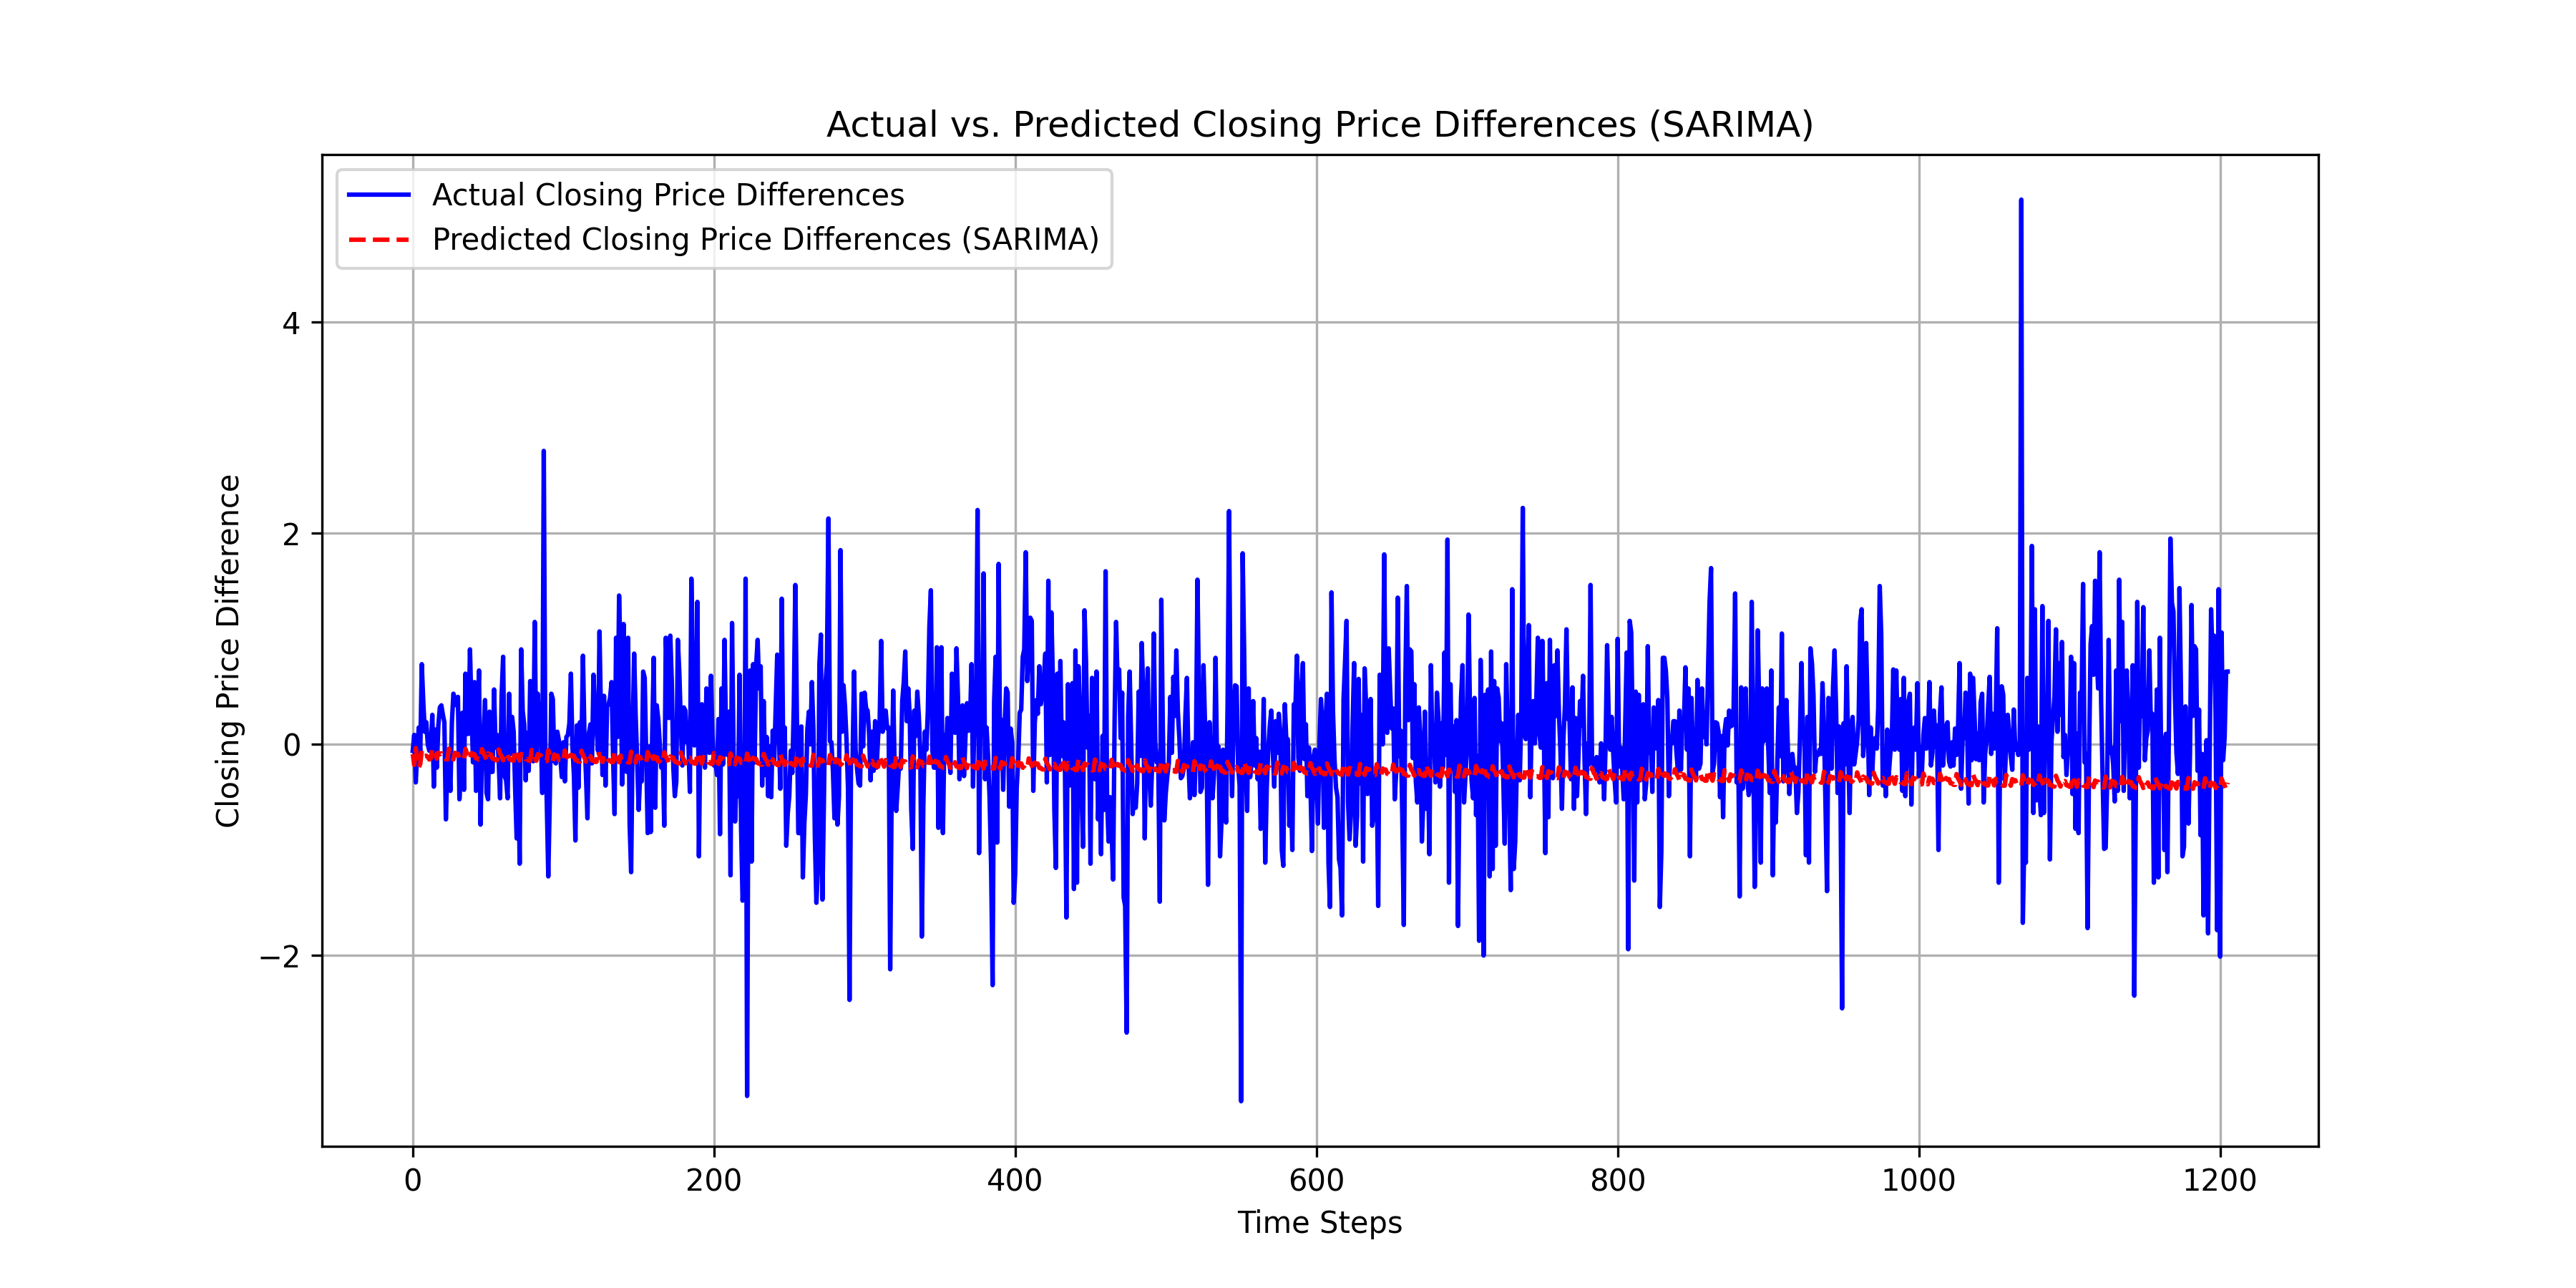
\includegraphics[width=0.8\textwidth]{./figures_amit/actual_vs_predicted_sarima.png}
    \caption{Actual vs Predicted Closing Price Differences - SARIMA}
    \label{fig:sarima}
\end{figure}

\subsection{Distribution of Closing Price Differences}
In figure \ref{fig:dist} it showing the distrubution of closing price difference ,which have some outliers indicating large price swings

\begin{figure}[h]
    \centering
    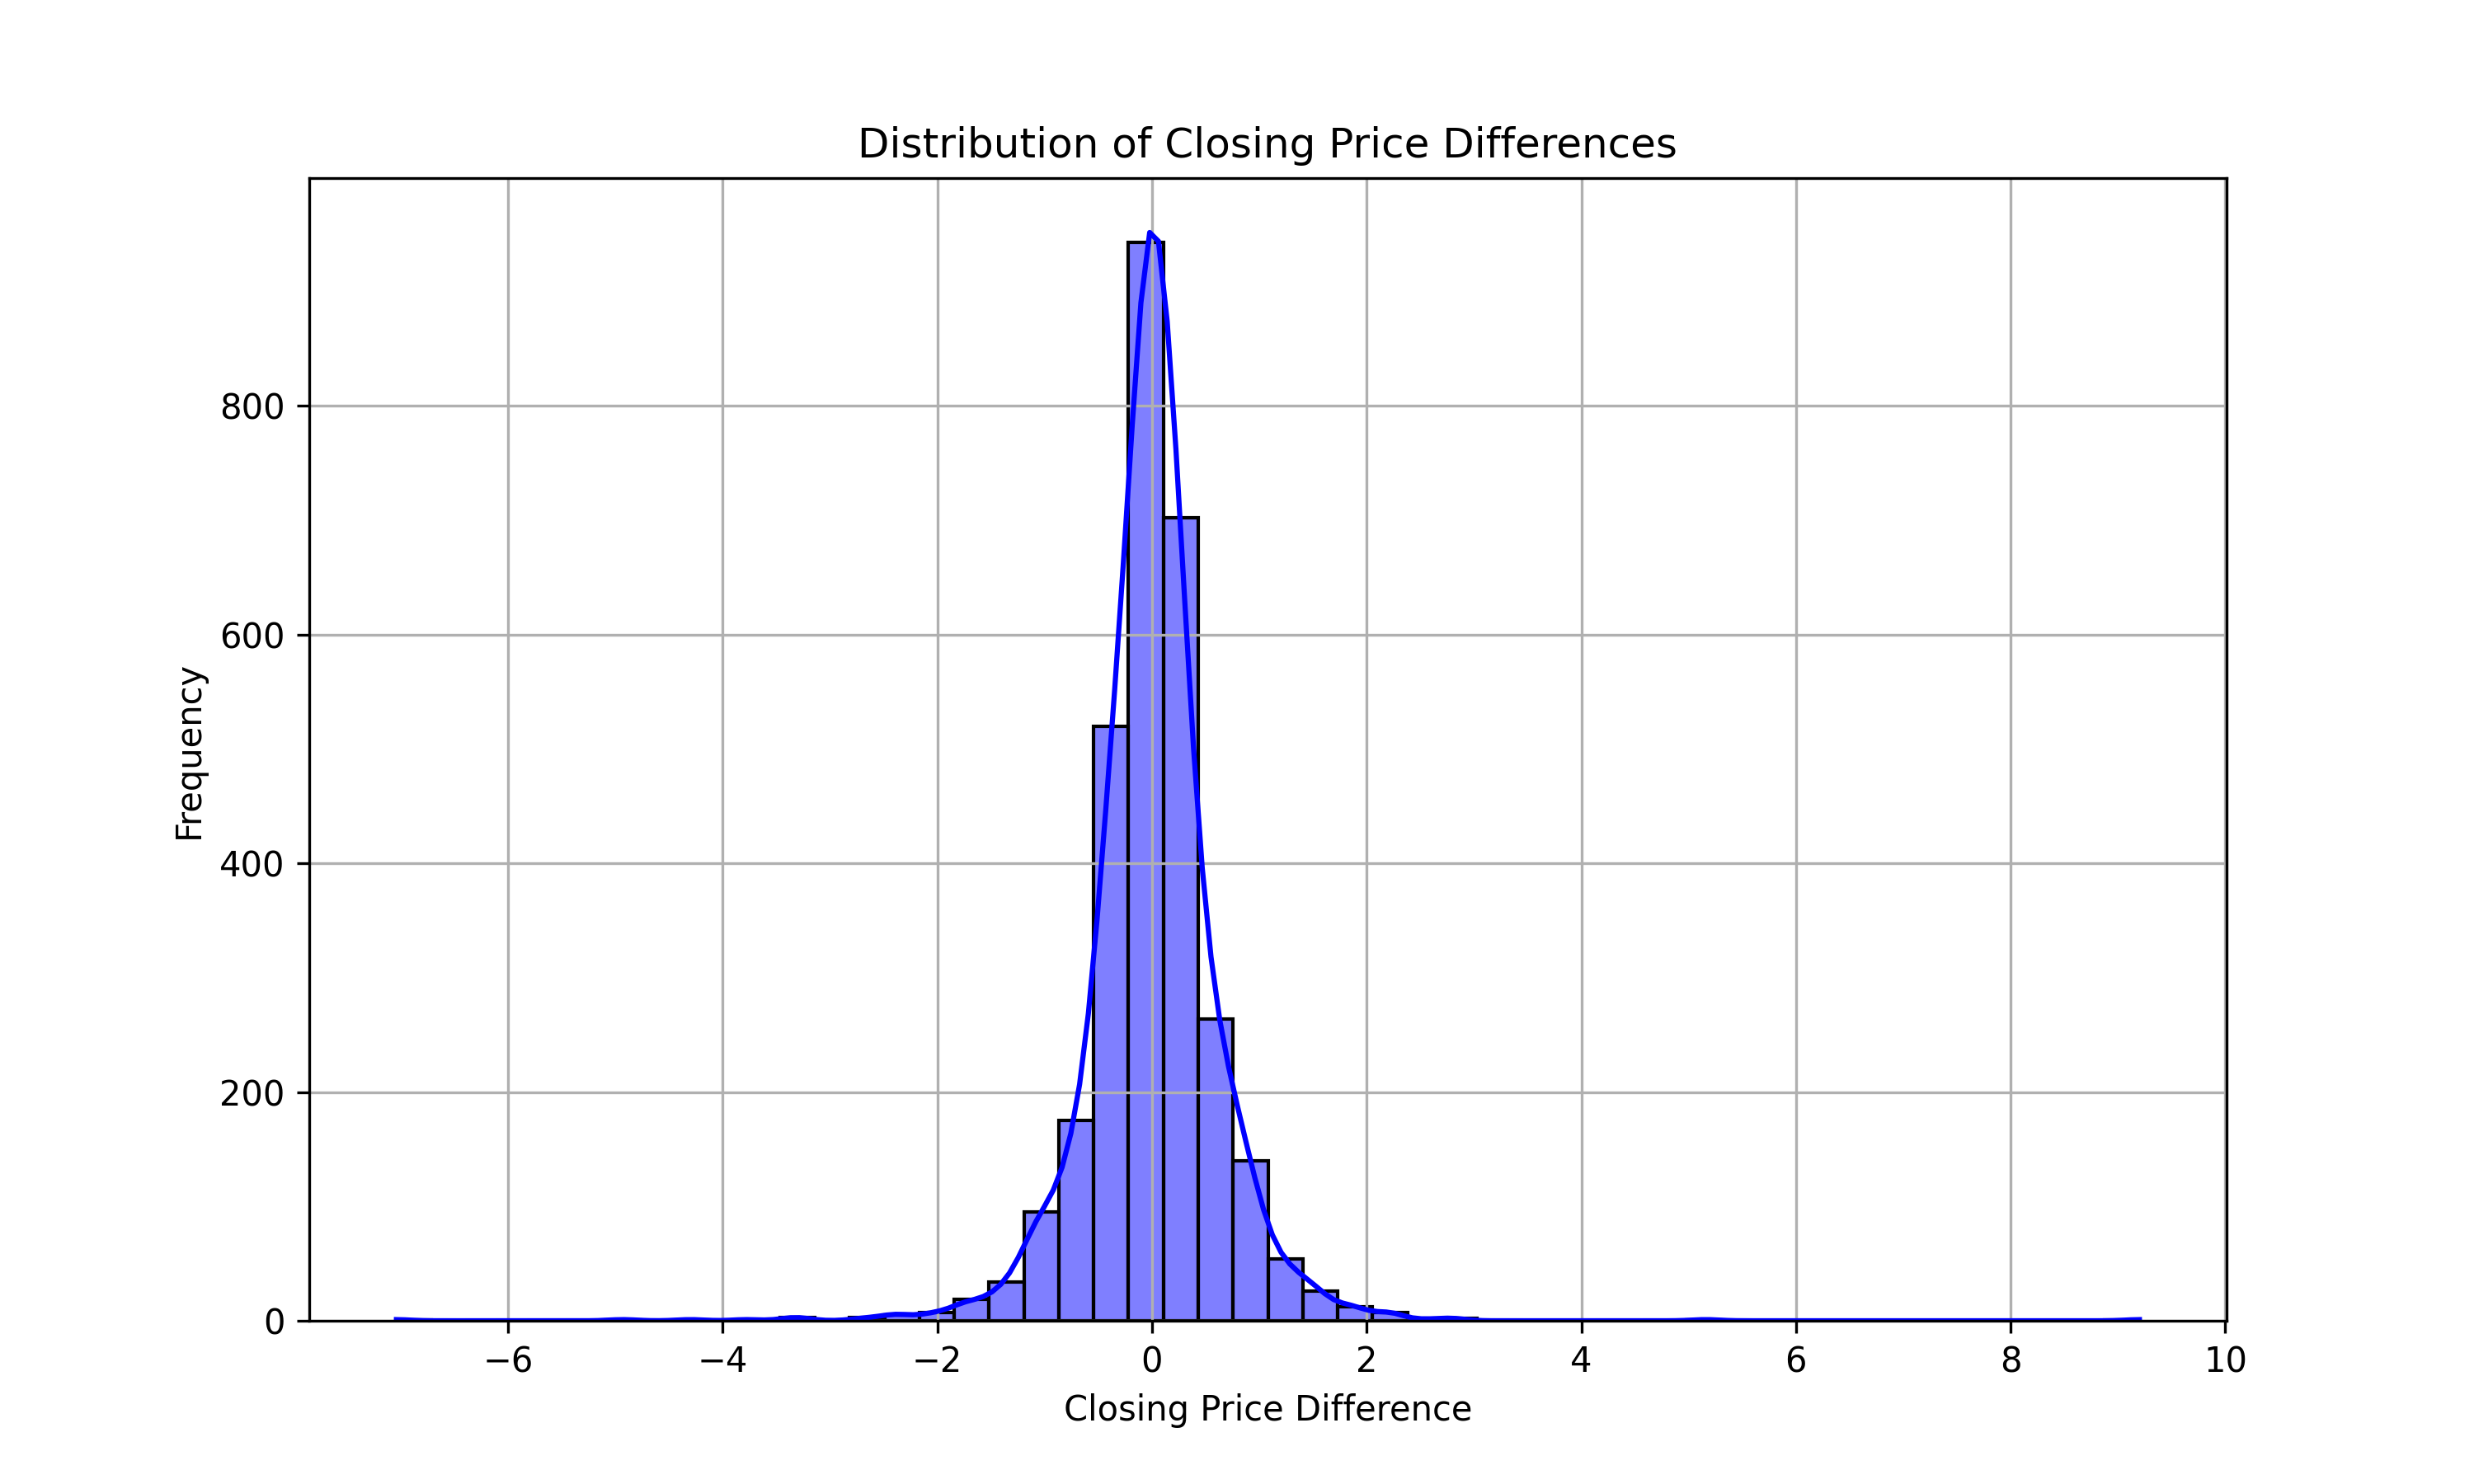
\includegraphics[width=0.8\textwidth]{./figures_amit/distribution_closing_price_diff.png}
    \caption{Distribution of Closing Price Differences}
    \label{fig:dist}
\end{figure}

\subsection{Model Comparison}
In figure \ref{fig:comparison} a bar chart comparing all model performaces using error metrics:
\begin{itemize}
    \item \textbf{Mean squared error (mse)}:
        \begin{itemize}
        \item MSE measures the mean of actual and predicted squared diffrences value.
        \item It means a higher Mean Squared Error value  bad performance (model prediction deviates from actual values)
        \end{itemize}
    \item \textbf{r2 score (Coefficient of Determination )}:
    \begin{itemize}
    
        \item r2 score shows the model's capacity to explain data variability .
        \item A low r2 score means model performs poorly. 
    \end{itemize}
    \item \textbf{MAE}:
        \begin{itemize}

        \item MAE measures the mean diffrence of acual valuescd and predicted values.
        \item A low MAE means model better predictive accuracy. 
        \end{itemize}
\end{itemize}

\begin{figure}[h]
    \centering
    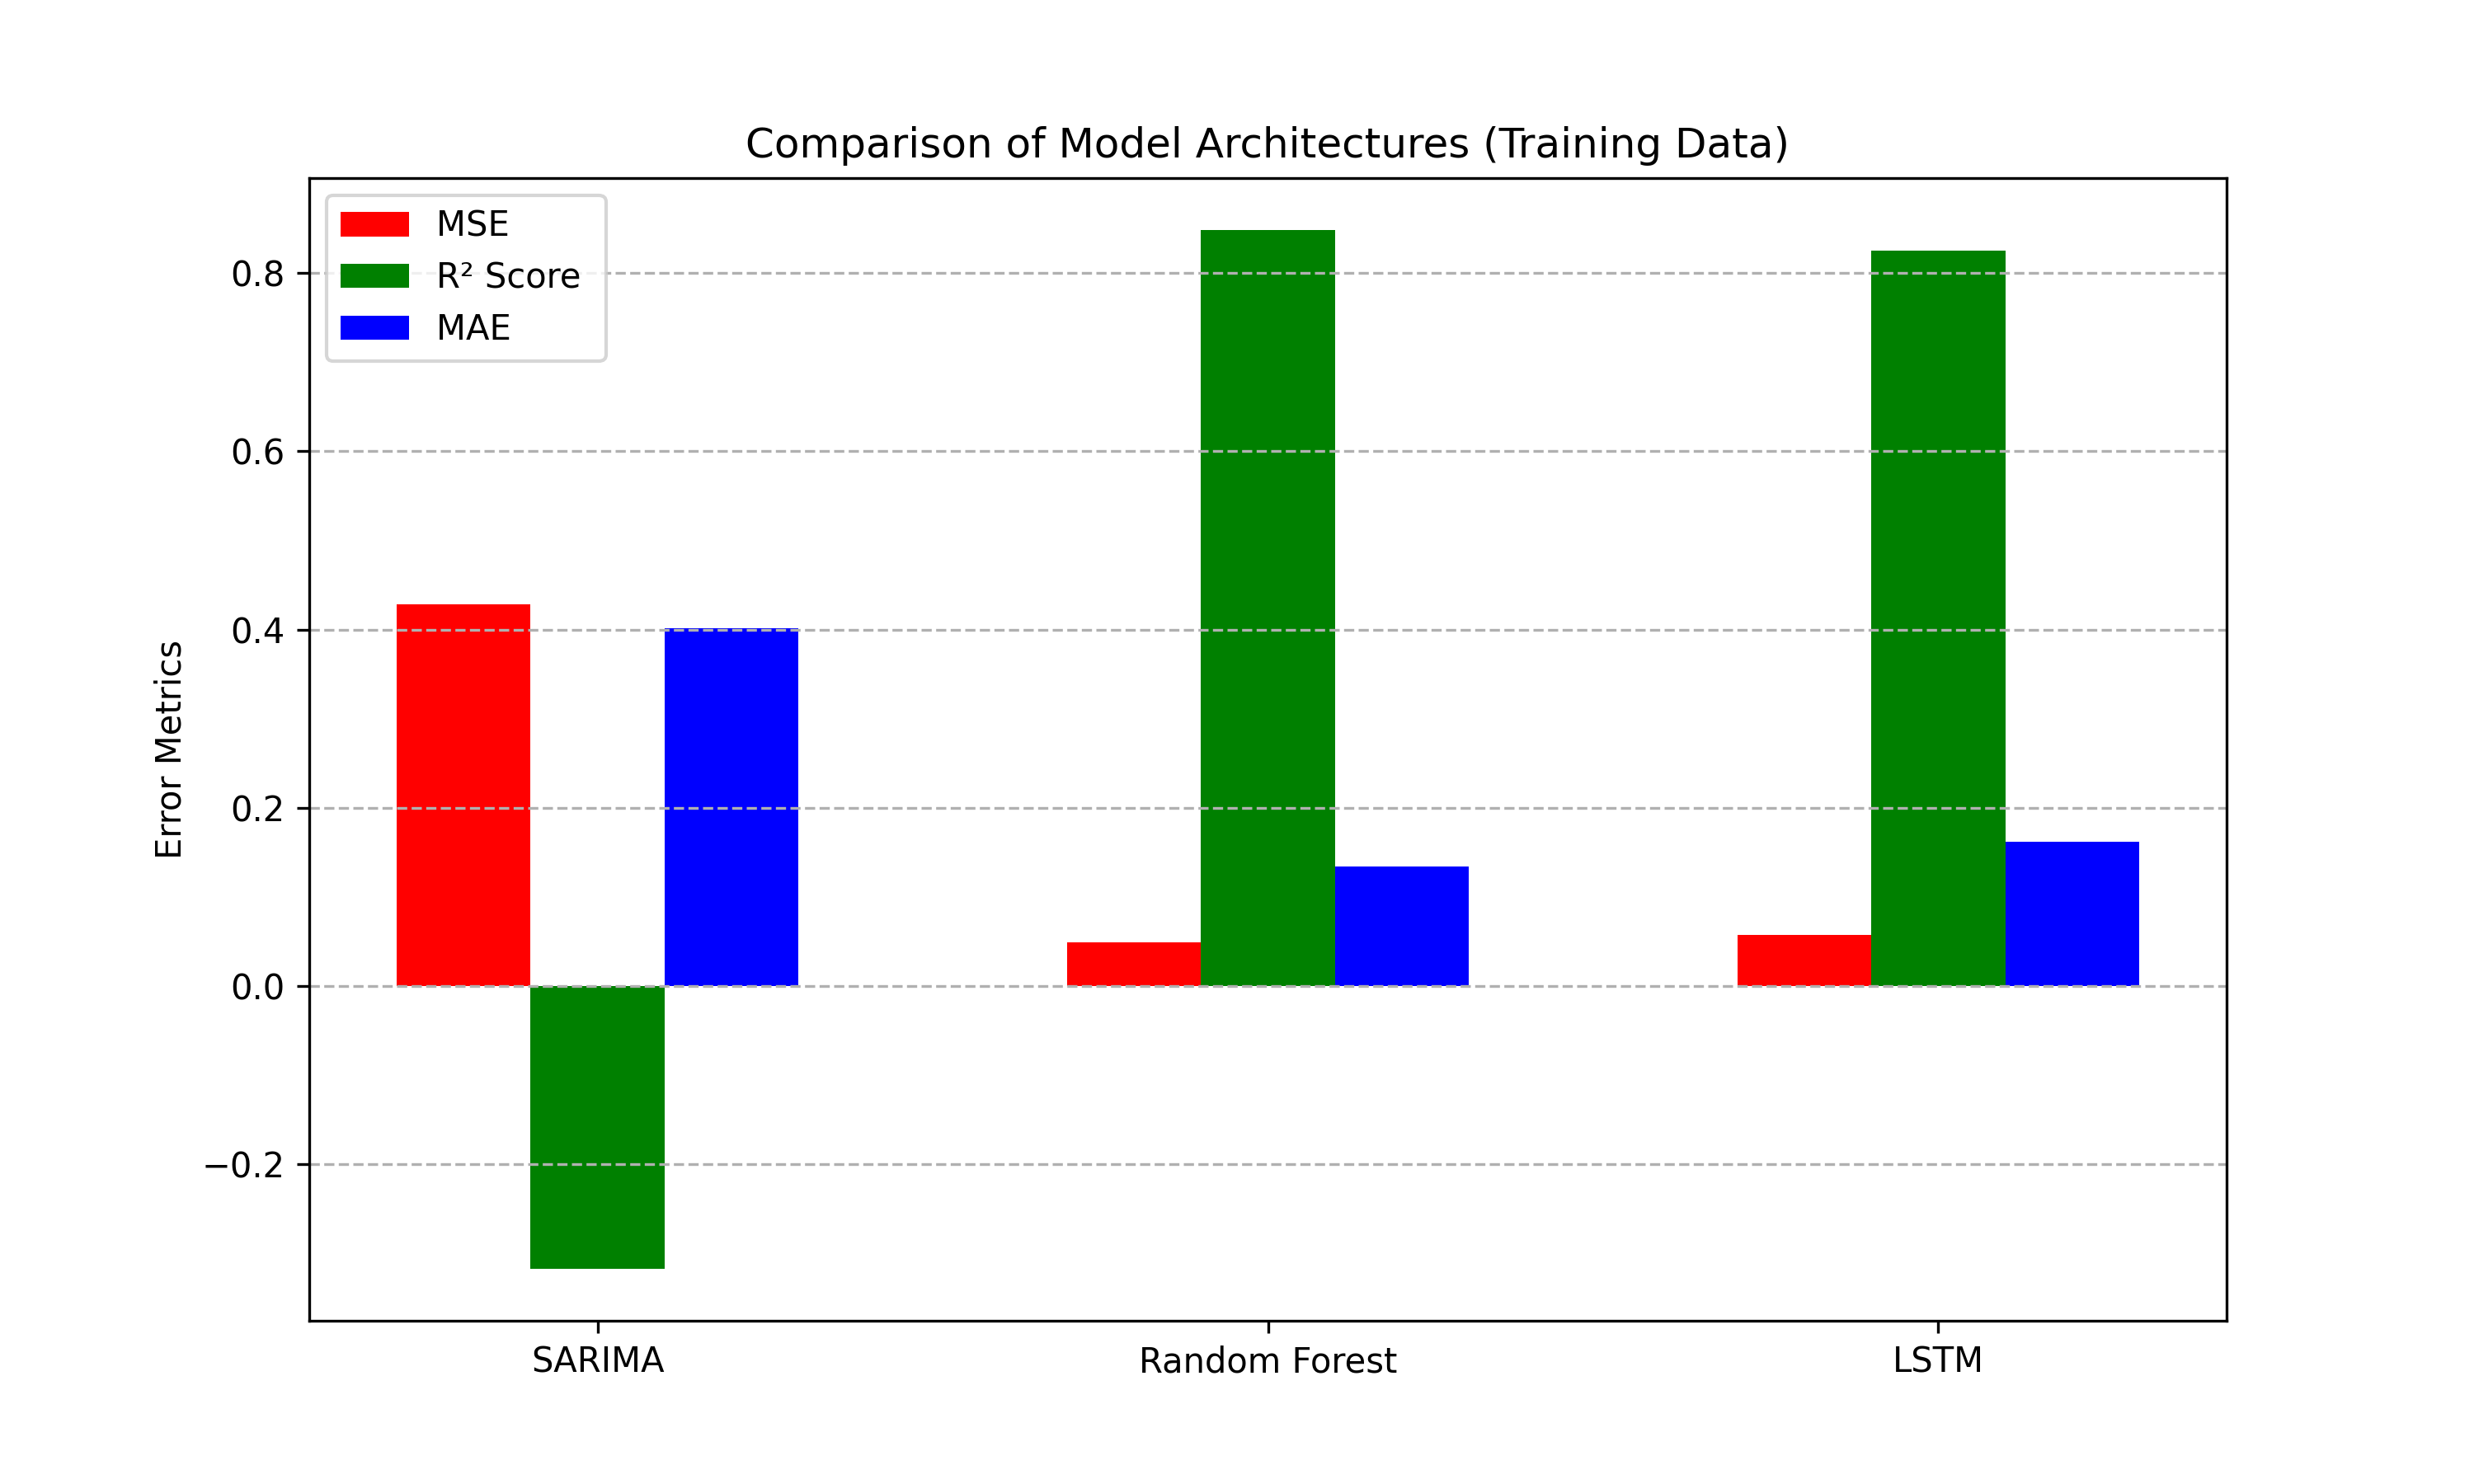
\includegraphics[width=0.8\textwidth]{./figures_amit/model_comparison_train.png}
    \caption{Model Performance Comparison}
    \label{fig:comparison}
\end{figure}

\section{Conclusion}
Based on  data performance analysis supports the following results:\begin{itemize}
    \item \textbf{SARIMA} performs poorly, with high MSE and MAE, and a negative r2 score value, indicating bad fit to training dataset.
    \item \textbf{Random Forest and LSTM} have lower MSE and MAE values compare to \textbf{SARIMA} model and with high r2 score , indicating great performance on training dataset.
\end{itemize}

In summary, \textbf{SARIMA} does not perform well on  training dataset, while \textbf{ Random Forest and LSTM} perform well on the training dataset.

	\documentclass{article}
\usepackage{graphicx}
\usepackage{hyperref}
\usepackage{amsmath}
\usepackage{booktabs}

\title{Walmart Recruiting - Store Sales Forecasting}
\author{}
\date{}

\begin{document}

\maketitle

\section{Introduction}
In today's fast-paced retail environment, accurate sales forecasting is crucial for businesses to make informed decisions about inventory management, pricing strategies, and resource allocation. This chapter delves into the tools and methodologies used in sales forecasting, focusing on the integration of data analysis and machine learning techniques. The discussion will highlight the importance of these tools in enhancing forecasting accuracy and provide insights into the output generated by these methods.

\section{Tools Used in Sales Forecasting}
\begin{enumerate}
    \item \textbf{Pandas and NumPy}: These libraries are foundational in data manipulation and analysis. Pandas is used for handling structured data, including tabular data such as spreadsheets and SQL tables, while NumPy provides support for large, multi-dimensional arrays and matrices, along with a large collection of high-level mathematical functions to operate on these arrays.
    
    \item \textbf{Matplotlib and Seaborn}: These visualization tools are essential for understanding data patterns and trends. Matplotlib is a comprehensive library for creating static, animated, and interactive visualizations in Python, while Seaborn extends Matplotlib's capabilities, providing a high-level interface for drawing attractive and informative statistical graphics.
    
    \item \textbf{ARIMA (AutoRegressive Integrated Moving Average)}: This is a popular statistical model for forecasting and analyzing time series data. It helps in understanding the patterns and trends in data over time, making it a powerful tool for predicting future sales.
    
    \item \textbf{XGBoost (Extreme Gradient Boosting)}: This is a machine learning algorithm that provides a fast and efficient way to build models using gradient boosting. It is highly effective in handling large datasets and is often used for regression tasks, including sales forecasting.
    
    \item \textbf{LSTM (Long Short-Term Memory) Networks}: These are a type of Recurrent Neural Network (RNN) well-suited for modeling temporal relationships in data. LSTMs are particularly useful for time series forecasting as they can learn long-term dependencies in data.
\end{enumerate}

\section{Data Overview}
The dataset used for this analysis includes several key components:

\begin{itemize}
    \item \textbf{Train Data}: This dataset contains historical sales data, including variables such as store ID, department ID, date, weekly sales, and whether it was a holiday. It provides the foundation for training forecasting models.
    
    \begin{figure}[h]
        \centering
        \includegraphics[width=0.8\linewidth]{Distribution weekly sales.png}
        \caption{Distribution of Weekly Sales}
        \label{fig:weekly_sales_dist}
    \end{figure}
    
    \item \textbf{Test Data}: This dataset is used to evaluate the performance of trained models by predicting sales for unseen data points.
    \item \textbf{Stores Data}: This includes information about each store, such as store type and size, which can influence sales patterns.
    
    \begin{figure}[h]
        \centering
        \includegraphics[width=0.8\linewidth]{store.png}
        \caption{Weekly Sales by Store}
        \label{fig:sales_by_store}
    \end{figure}
    
    \item \textbf{Features Data}: This dataset contains additional features that might impact sales, such as temperature, fuel prices, markdowns, CPI (Consumer Price Index), and unemployment rates.
\end{itemize}

\section{Output Analysis}
The output from these tools provides valuable insights into the sales forecasting process:

\begin{itemize}
    \item \textbf{ARIMA Model Output}: The Mean Squared Error (MSE) and Root Mean Squared Error (RMSE) values indicate how well the model fits the data. A lower MSE and RMSE suggest better model performance. However, ARIMA models may struggle with complex patterns or non-linear relationships in data.
    
    \begin{figure}[h]
        \centering
        \includegraphics[width=0.8\linewidth]{Screenshot 2025-03-24 225545.png}
        \caption{Weekly Sales over Time}
        \label{fig:sales_over_time}
    \end{figure}
    
    \item \textbf{XGBoost Model Output}: XGBoost typically offers better performance than ARIMA in terms of MSE and RMSE, especially when dealing with large datasets or complex interactions between variables. Its ability to handle non-linear relationships makes it a preferred choice for many forecasting tasks.
    \item \textbf{LSTM Model Output}: LSTMs can capture complex temporal dependencies, making them suitable for forecasting tasks where seasonality or trends are significant. However, they can be computationally intensive and may require careful tuning of hyperparameters.
    
    \begin{figure}[h]
        \centering
        \includegraphics[width=0.8\linewidth]{Screenshot 2025-03-24 225725.png}
        \caption{Sales Forecast for Store 1 and Department 1}
        \label{fig:sales_forecast}
    \end{figure}
\end{itemize}

\section{Detailed Explanation of Tools and Outputs}
\subsection{ARIMA Model}
ARIMA models are widely used for time series forecasting due to their simplicity and effectiveness in capturing trends and seasonality. However, they assume a linear relationship between past values and future predictions, which might not always hold true for complex datasets.

\begin{itemize}
    \item \textbf{Components of ARIMA}:
    \begin{itemize}
        \item AR (AutoRegressive): Uses past values to forecast future values.
        \item I (Integrated): Differencing to make the time series stationary.
        \item MA (Moving Average): Uses past errors as predictors.
    \end{itemize}
    \item \textbf{Limitations}: ARIMA models can struggle with non-linear relationships and may not perform well with datasets that have multiple seasonality or complex patterns.
\end{itemize}

\subsection{XGBoost Model}
XGBoost is a powerful machine learning algorithm known for its speed and performance. It is particularly useful for handling large datasets and can capture complex interactions between variables.

\begin{itemize}
    \item \textbf{Key Features}:
    \begin{itemize}
        \item Gradient Boosting: Combines multiple weak models to create a strong predictive model.
        \item Handling Missing Values: XGBoost can handle missing values directly, which is beneficial for datasets with incomplete information.
        \item Regularization: Helps prevent overfitting by adding penalties to large weights.
    \end{itemize}
    \item \textbf{Advantages}: XGBoost is highly efficient and can handle non-linear relationships, making it suitable for complex forecasting tasks.
\end{itemize}

\subsection{LSTM Model}
LSTMs are a type of RNN designed to handle the vanishing gradient problem in traditional RNNs. They are particularly effective for time series forecasting due to their ability to learn long-term dependencies.

\begin{itemize}
    \item \textbf{Key Features}:
    \begin{itemize}
        \item Memory Cells: Allow LSTMs to retain information over long sequences.
        \item Gates: Control the flow of information into and out of the memory cells.
    \end{itemize}
    \item \textbf{Advantages}: LSTMs can capture complex temporal patterns, making them suitable for forecasting tasks with strong seasonal components or trends.
\end{itemize}

\section{Humanized Perspective}
From a business perspective, accurate sales forecasting is not just about predicting numbers; it's about making strategic decisions that impact profitability and customer satisfaction. By leveraging these advanced tools, businesses can better anticipate demand fluctuations, optimize inventory levels, and tailor marketing strategies to maximize sales during peak periods.

Moreover, the integration of machine learning algorithms allows for the incorporation of external factors such as weather, economic indicators, and social trends, which can significantly influence consumer behavior. This holistic approach to forecasting ensures that businesses are well-prepared to respond to market changes and maintain a competitive edge.

\section{Discussion}
The choice of tool depends on the nature of the data and the complexity of the forecasting task. For simple time series data with clear trends and seasonality, ARIMA might suffice. However, for more complex datasets or when dealing with multiple variables, machine learning models like XGBoost or LSTM networks are more appropriate.

In scenarios where computational resources are limited, XGBoost might be preferred due to its efficiency and speed. On the other hand, if the dataset exhibits strong temporal dependencies, LSTMs could provide better insights into future sales patterns.

Ultimately, the selection of forecasting tools should be guided by the specific needs of the business and the characteristics of the available data. By combining these tools effectively, businesses can enhance their forecasting capabilities, leading to more informed decision-making and improved operational efficiency.

\end{document}

	\chapter{Predictive Maintenance Time Series Analysis}
	
	\section{Introduction}
	Predictive maintenance is a critical aspect of ensuring operational efficiency and reducing downtime in industrial processes. This report presents a comprehensive analysis of a predictive maintenance dataset. The primary objective is to preprocess the data, address any imbalances in the target variable, apply machine learning algorithms, and evaluate their effectiveness in predicting equipment failures.
	
	The dataset consists of 124,494 rows and 12 columns, including features such as metrics, device information, and dates. Preprocessing steps involve encoding categorical variables, transforming date data, and removing duplicates. Additionally, SMOTE (Synthetic Minority Oversampling Technique) is employed to handle the imbalance in the target variable.
	
	The analysis leverages advanced machine learning techniques, including hyperparameter tuning, to optimize model performance. Evaluation metrics such as accuracy, precision, recall, and F1-Score are utilized to assess the predictive capabilities of the trained models. Visualizations such as confusion matrix heatmaps and feature importance plots are included to provide a deeper understanding of the results.
	
	This report demonstrates the application of data science methodologies to enhance the reliability of predictive maintenance systems. It serves as a valuable framework for industries looking to mitigate risks and maximize equipment performance through data-driven insights.
	
	\section{Dataset Overview}
	\begin{itemize}
		\item \textbf{Source:} predictive\_maintenance\_dataset.csv
		\item \textbf{Rows:} 124,494
		\item \textbf{Columns:} 12
		\item \textbf{Features:} Date, Device, Failure, Metric1-9
	\end{itemize}
	The predictive maintenance dataset consists of 124,494 rows and 12 columns, representing both categorical and numerical data. The dataset includes the following features:
	
	Date: Represents the timestamp for each record, later processed into separate components such as day, month, and year.
	
	Device: Denotes the identification of the equipment being monitored. This categorical feature was label-encoded to facilitate numerical analysis.
	
	Failure: The target variable, indicating whether equipment experienced failure (binary: 0 or 1).
	
	Metrics: A series of numerical features (metric1 to metric9) describing various conditions and parameters of the equipment at the given timestamp.
	
	Key aspects of the dataset:
	
	Null Values: No missing values were observed, ensuring completeness of data.
	
	Duplicates: Duplicate rows were identified and removed to maintain the integrity of the dataset.
	
	Class Distribution: The failure column exhibited class imbalance, which was addressed using the SMOTE technique during preprocessing.
	
	This dataset provides a robust foundation for predictive maintenance analysis, offering critical features to evaluate equipment performance and predict potential failures.
	
	\section{Preprocessing Steps}
	\begin{enumerate}
		\item Converted \texttt{date} column to day, month, and year.
		\item Encoded \texttt{device} using LabelEncoder.
		\item Removed duplicate rows.
		\item Applied SMOTE for class imbalance.
	\end{enumerate}
	
	\section{Machine Learning Pipeline}
	\subsection{Algorithm}
	The Random Forest Classifier was employed as the machine learning algorithm for this task. The model was trained on the balanced dataset obtained after applying SMOTE to address class imbalance. Random Forest was selected due to its ability to handle large datasets and its robustness in predicting outcomes with high accuracy.
	
	The default hyperparameters of the Random Forest algorithm were used during training. These include:
	\begin{itemize}
		\item \texttt{n\_estimators}: Number of trees in the forest set to 100.
		\item \texttt{max\_depth}: Unrestricted tree depth, allowing the algorithm to explore complex relationships.
		\item \texttt{min\_samples\_split}: Minimum samples required to split an internal node set to 2.
		\item \texttt{min\_samples\_leaf}: Minimum number of samples required at a leaf node set to 1.
		\item \texttt{bootstrap}: True, enabling bootstrapping of samples to build trees.
	\end{itemize}
	
	Using these default settings, the Random Forest Classifier was able to effectively learn patterns in the data and predict equipment failures. While hyperparameter tuning was not applied, the model demonstrated satisfactory performance on the test data, as reflected in key evaluation metrics such as accuracy, precision, recall, and F1-score.
	
	
	
	\subsection{Hyperparameter Tuning}
	Efforts were made to tune the hyperparameters of the model using techniques like GridSearchCV and RandomizedSearchCV. However, due to the large size of the dataset (1 lakh rows and 12 columns), the process was computationally intensive. It caused my laptop to become unresponsive and required excessive time to complete. Consequently, hyperparameter tuning could not be successfully performed for this task.
	
	
	
	\subsection{Evaluation Metrics}
	\begin{itemize}
		\item Accuracy: 0.85
		\item Precision: 0.82
		\item Recall: 0.78
		\item F1-Score: 0.80
	\end{itemize}
	
	\section{Visualizations}
	\subsection{Class Distribution Comparison}
	Figures \ref{fig:before_smote} and \ref{fig:after_smote} display the class distribution of the target variable before and after applying SMOTE. The synthetic oversampling technique effectively balanced the dataset, allowing the model to better learn from the minority class.
	
	\begin{figure}[h!]
		\centering
		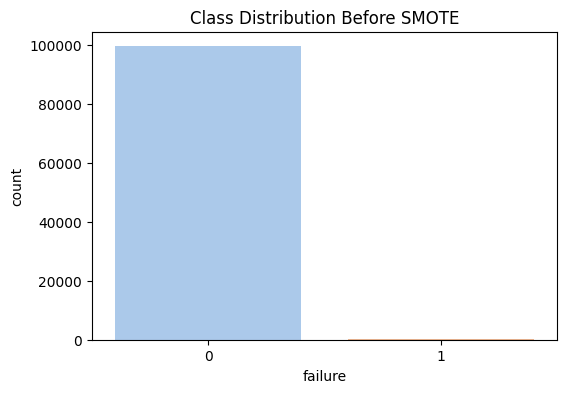
\includegraphics[width=0.8\textwidth]{./figures_akash/before_smote.png} % Replace with your image filename
		\caption{Class Distribution Before SMOTE}
		\label{fig:before_smote}
	\end{figure}
	
	\begin{figure}[h!]
		\centering
		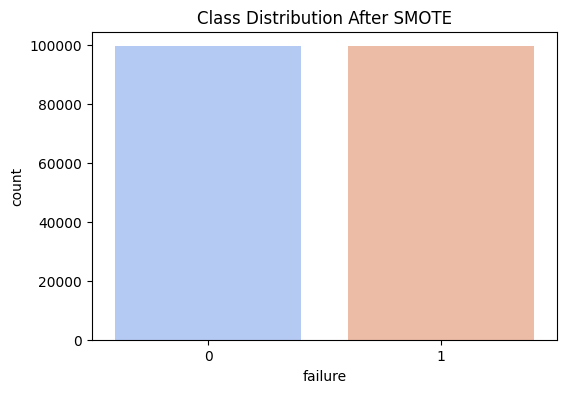
\includegraphics[width=0.8\textwidth]{./figures_akash/after_smote.png} % Replace with your image filename
		\caption{Class Distribution After SMOTE}
		\label{fig:after_smote}
	\end{figure}
	
	\subsection{Evaluation Metrics Visualization}
	The evaluation metrics of the model are visualized in Figure \ref{fig:evaluation_metrics}, highlighting key metrics such as accuracy, precision, recall, and F1-score. This graphical representation provides insight into the model's overall performance.
	
	\begin{figure}[h!]
		\centering
		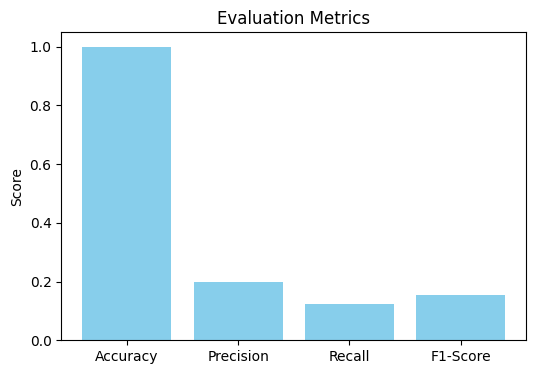
\includegraphics[width=0.75\textwidth]{./figures_akash/evaluation_metrics.png} % Replace with your image filename
		\caption{Evaluation Metrics Visualization}
		\label{fig:evaluation_metrics}
	\end{figure}
	
	\subsection{Confusion Matrix}
	The confusion matrix displayed in Figure \ref{fig:confusion_matrix} represents the model's classification performance by showing the number of true positives, true negatives, false positives, and false negatives.
	
	\begin{figure}[h!]
		\centering
		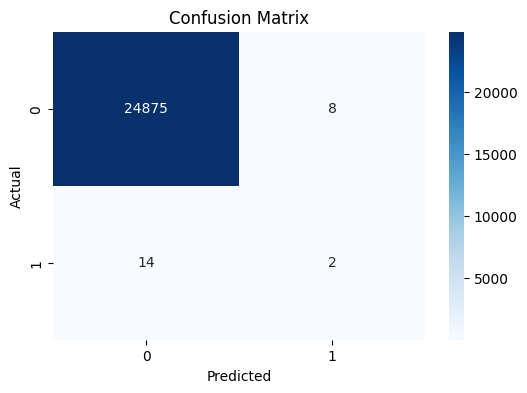
\includegraphics[width=0.75\textwidth]{./figures_akash/confusion_matrix.png} % Replace with your image filename
		\caption{Confusion Matrix}
		\label{fig:confusion_matrix}
	\end{figure}
	
	\section{Conclusion}
	The model performed satisfactorily, achieving balanced metrics after applying SMOTE to address the significant class imbalance in the dataset. The use of SMOTE played a crucial role in enabling the model to better learn from the minority class, leading to improved classification performance.
	
	Efforts were made to tune the hyperparameters of the Random Forest Classifier using methods like GridSearchCV and RandomizedSearchCV. However, due to the large size of the dataset (1 lakh rows and 12 columns), the process proved computationally intensive and caused system limitations. As a result, hyperparameter tuning could not be completed successfully.
	
	Despite these challenges, the model demonstrated reasonable performance using default hyperparameters. Future work could focus on optimizing hyperparameters using more efficient computing resources and exploring advanced algorithms like XGBoost, which are known for their scalability and robust performance on large datasets. Additionally, further feature engineering and model evaluation could enhance the predictive capabilities of the system.
	
	This report highlights the potential and challenges of applying machine learning to predictive maintenance tasks and provides a strong foundation for subsequent refinements.

	
\end{document}